\pdfoutput=1
\documentclass[acmsmall,screen,10pt]{acmart} % anonymous, review
\settopmatter{printfolios=true,printacmref=false}
\acmConference[ICFP 2020]{International Conference on Functional Programming}{24 -- 26 August 2020}{Jersey City, NJ, United States}

\title{Practical Sized Typing for Coq}

\author{Jonathan Chan}
\orcid{0000-0003-0830-3180}
\affiliation{
  \institution{University of British Columbia}
}
\email{jon@alumni.ubc.ca}

\author{William J. Bowman}
\orcid{0000-0002-6402-4840}
\affiliation{
  \institution{University of British Columbia}
}
\email{wilbowma@cs.ubc.ca}

% Fixes for arXiv submission
% Fix `Undefined control sequence. <argument> \mdseries@tt`
\makeatletter
\providecommand{\mdseries@tt}{}
\makeatother

\usepackage{tikz}
\usetikzlibrary{shapes,arrows}
\usepackage{amsmath}
\usepackage{amsfonts}
\usepackage{mathtools}
\usepackage{stmaryrd}
\usepackage[frozencache,cachedir=.]{minted}
\usepackage{bussproofs}
\usepackage{mathpartir}
\usepackage{xspace}
\usepackage[shortcuts]{extdash}
\usepackage{enumitem}
\usepackage[title]{appendix}
\usepackage{proof}
\usepackage{doi}

% Use \autoref for references with prefixes
\def\sectionautorefname{Section}
\def\subsectionautorefname{Subsection}
\def\subsubsectionautorefname{Subsubsection}
\def\figureautorefname{Figure}
\def\tableautorefname{Table}
\def\Appendixautorefname{Appendix}
% Force upright style in mathpartir inferrule* right label
\renewcommand{\RightTirNameStyle}{\upshape}
% Shrink bibliography font size
%\renewcommand*{\bibfont}{\small}
% Get rid of first page first column footnote conference information
\renewcommand\footnotetextcopyrightpermission[1]{}
% Get rid of headers/footers
\makeatletter
\fancypagestyle{firstpagestyle}{
    \fancyhf{}
    \fancyhead[LO]{\ACM@linecountL}
    \fancyhead[RO]{\@folioblob}
    \fancyheadoffset[RO,LE]{0.6\@folio@wd}
    \fancyfoot{}
}
\makeatother
\fancyfoot{}
%\fancyhead[L]{\shorttitle}
%\fancyhead[R]{\shortauthors}

% rule hyperlinks
\newcommand{\defrule}[1]{\phantomsection\label{#1}(\text{#1})}
\newcommand{\defnamerule}[2]{\phantomsection\label{#1}(#2)}
\newcommand{\refrule}[1]{\hyperref[#1]{Rule (#1)}}
\newcommand{\refnorule}[1]{\hyperref[#1]{(#1)}}
% langs
\newcommand{\lang}{CIC$\widehat{*}$\xspace}
\newcommand{\titlelang}{\texorpdfstring{\lang}{CIC\^{}*}\xspace}
\newcommand{\CIChat}{CIC$\widehat{~}$\xspace}
\newcommand{\CIChatbar}{CIC$\widehat{\text{\underline{\:\:}}}$\xspace}
\newcommand{\Fhat}{F$\widehat{~}$\xspace}
\newcommand{\CIChatl}{CIC$\widehat{_l}$\xspace}
\newcommand{\CChatomega}{CC$\widehat{\omega}$\xspace}
\newcommand{\CIChatsub}{CIC$\widehat{_\sqsubseteq}$\xspace}
% metafunctions (for math envs)
\newcommand{\dom}[1]{\text{dom}(#1)}
\newcommand{\SV}[1]{\text{SV}(#1)}
\newcommand{\WF}[1]{\text{WF}(#1)}
\newcommand{\whnf}[1]{\textsc{whnf}(#1)}
\newcommand{\fresh}[1]{\textsc{fresh}(#1)}
\newcommand{\freshi}[1]{\textsc{fresh*}(#1)}
\newcommand{\axiom}[1]{\textsc{axiom}(#1)}
\newcommand{\rules}[2]{\textsc{rule}(#1, #2)}
\newcommand{\elim}[3]{\textsc{elim}(#1, #2, #3)}
\newcommand{\inds}[1]{\textsc{inds}(#1)}
\newcommand{\indtype}[2]{\textsc{indType}(#1, #2)}
\newcommand{\constrtype}[3]{\textsc{constrType}(#1, #2, #3)}
\newcommand{\motivetype}[4]{\textsc{motiveType}(#1, #2, #3, #4)}
\newcommand{\branchtype}[5]{\textsc{branchType}(#1, #2, #3, #4, #5)}
\newcommand{\indsig}[1]{\textsc{indSig}(#1)}
\newcommand{\constrsig}[1]{\textsc{constrSig}(#1)}
\newcommand{\caseStage}[2]{\textsc{caseStage}(#1, #2)}
\newcommand{\decompose}[2]{\textsc{decompose}(#1, #2)}
\newcommand{\shift}[1]{\textsc{shift}(#1)}
\newcommand{\setrecstars}[2]{\textsc{setRecStars}(#1, #2)}
\newcommand{\setcorecstars}[1]{\textsc{setCorecStars}(#1)}
\newcommand{\getrecvar}[2]{\textsc{getRecVar}(#1, #2)}
\newcommand{\getcorecvar}[1]{\textsc{getCorecVar}(#1)}
\newcommand{\getposvars}[2]{\textsc{getPosVars}(#1, #2)}
\newcommand{\RecCheckLoop}[4]{\textsc{RecCheckLoop}(#1, #2, #3, #4)}
% terms (for math envs)
\newcommand{\Prop}{\text{Prop}}
\newcommand{\Set}{\text{Set}}
\newcommand{\Type}[1]{\text{Type}_{#1}}
\newcommand{\letin}[4]{\text{let}\ #1 : #2 \coloneqq #3\ \text{in}\ #4}
\newcommand{\caseof}[4]{\text{case}_{#1}\ #2\ \text{of}\ \langle #3 \Rightarrow #4 \rangle}
\makeatletter
    \def\fix{\@ifstar{\@@fix}{\@fix}}
    \def\cofix{\@ifstar{\@@cofix}{\@cofix}}
    \newcommand{\@fix}[4]{\text{fix}_{#1}\ \langle #2 : #3 \coloneqq #4 \rangle}
    \newcommand{\@cofix}[4]{\text{cofix}_{#1}\ \langle #2 : #3 \coloneqq #4 \rangle}
    \newcommand{\@@fix}[4]{\text{fix}_{#1}\ #2 : #3 \coloneqq #4}
    \newcommand{\@@cofix}[4]{\text{cofix}_{#1}\ #2 : #3 \coloneqq #4}
\makeatother
\newcommand{\Size}{\text{Size}}
\newcommand{\SizeLt}{\text{Size<}}
\newcommand{\SizeUniv}{\text{SizeUniv}}
% other (for math envs)
\newcommand{\set}[1]{\{#1\}}
\newcommand{\sgg}{\Sigma, \Gamma_G, \Gamma}
\newcommand{\cgg}{C, \Gamma_G, \Gamma}
\newcommand{\pos}{\ \text{pos}\ }
\renewcommand{\neg}{\ \text{neg}\ }
% other
\newcommand{\inmaterials}{in the anonymous supplementary materials}
\newcommand{\spacer}{\vspace{1ex}}
% (co) words
\newcommand{\coinductive}{(co)\-inductive\xspace}
\newcommand{\corecursive}{(co)\-recursive\xspace}
\newcommand{\cofixpoint}{(co)\-fix\-point\xspace}
\newcommand{\cofixpoints}{(co)\-fix\-points\xspace}

\begin{document}

\begin{abstract}
Termination of recursive functions and productivity of corecursive functions are important for maintaining logical consistency in proof assistants. However, contemporary proof assistants, such as Coq, rely on syntactic criteria that prevent users from easily writing obviously terminating or productive programs, such as quicksort. This is troublesome, since there exist theories for type-based termination- and productivity-checking.

In this paper, we present a design and implementation of sized type checking and inference for Coq. We extend past work on sized types for the Calculus of (Co)\-Inductive Constructions (CIC) with support for global definitions found in Gallina, and extend the sized-type inference algorithm to support completely unannotated Gallina terms. This allows our design to maintain complete backward compatibility with existing Coq developments. We provide an implementation that extends the Coq kernel with optional support for sized types.
\end{abstract}

\maketitle

\section{Introduction}\label{sec:intro}

Proof assistants based on dependent type theory rely on the termination of recursive functions and the productivity of corecursive functions to ensure two important properties: logical consistency, so that it is not possible to prove false propositions; and decidability of type checking, so that checking that a program proves a given proposition is decidable.

In the proof assistant Coq, termination and productivity are enforced by a \textit{guard predicate} on fixpoints and cofixpoints respectively. For fixpoints, recursive calls must be \textit{guarded by destructors}; that is, they must be performed on structurally smaller arguments. For cofixpoints, corecursive calls must be \textit{guarded by constructors}; that is, they must be the structural arguments of a constructor. The following examples illustrate these structural conditions.

\begin{minted}{coq}
Fixpoint add n m : nat :=
  match n with
  | O => m
  | S p => S (add p m)
  end.
Variable A : Type.
CoFixpoint const a : Stream A := Cons a (const a).
\end{minted}

In the recursive call to \texttt{add}, the first argument \texttt{p} is structurally smaller than \texttt{S p}, which is the form of the original first argument \texttt{n}. Similarly, in \texttt{const}, the constructor \texttt{Cons} is applied to the corecursive call.

The actual implementation of the guard predicate extends beyond the guarded\-/by\-/destructors and guarded\-/by\-/constructors conditions to accept a larger set of terminating and productive functions. In particular, function calls will be unfolded (i.e. inlined) in the bodies of \cofixpoints as needed before checking the guard predicate. This has a few disadvantages: firstly, the bodies of these functions are required, which hinders modular design; and secondly, the \cofixpoint bodies may become very large after unfolding, which can decrease the performance of type checking.

Furthermore, changes in the structural form of functions used in \cofixpoints can cause the guard predicate to reject the program even if the functions still behave the same. The following simple example, while artificial, illustrates this structural fragility.

\begin{minted}{coq}
Fixpoint minus n m :=
  match n, m with
  | O, _ => n
  | _, O => n
  | S n', S m' => minus n' m'
  end.
Fixpoint div n m :=
  match n with
  | O => O
  | S n' => S (div (minus n' m) m)
  end.
\end{minted}

If we replace \texttt{| O, \_ => n} with \texttt{| O, \_ => O} in \texttt{minus}, it does not change its behaviour, but since it can return \texttt{O} which is not a structurally-smaller term of \texttt{n} in the recursive call to \texttt{div}, the guard predicate is no longer satisfied. The acceptance of \texttt{div} then depends on a function external to it, which can lead to difficulty in debugging for larger programs. Furthermore, the guard predicate is unaware of the obvious fact that \texttt{minus} never returns a \texttt{nat} larger than its first argument, which the user would have to write a proof for in order for \texttt{div} to be accepted with our alternate definition of \texttt{minus}.

An alternative to guard predicates for termination and productivity enforcement uses \textit{sized types}. In essence, \coinductive types are annotated with a size annotation, which follows a simple size algebra: $s \coloneqq \upsilon \mid \hat{s} \mid \infty$, where $\upsilon$ ranges over size variables. If some object has size $s$, then the object wrapped in a constructor would have a successor size $\hat{s}$. For instance, the \texttt{nat} constructors follow the below rules:

\begin{center}
\bottomAlignProof
\AxiomC{}
\UnaryInfC{$\Gamma \vdash \text{O} : \text{Nat}^{\hat{s}}$}
\DisplayProof
\quad
\bottomAlignProof
\AxiomC{$\Gamma \vdash n : \text{Nat}^s$}
\UnaryInfC{$\Gamma \vdash \text{S}\ n : \text{Nat}^{\hat{s}} $}
\DisplayProof
\end{center}

Termination- and productivity-checking is then simply a type-checking rule that uses size information. For termination, the type of the function of the recursive call must have a smaller size than that of the outer fixpoint; for productivity, the outer cofixpoint must have a larger size than that of the function of the corecursive call. In short, they both follow the following (simplified) typing rule.

\begin{center}
\AxiomC{$\Gamma (f:t^\upsilon) \vdash e: t^{\hat{\upsilon}}$}
\UnaryInfC{$\Gamma \vdash \text{(co)fix}\ f : t := e : t^s$}
\DisplayProof
\end{center}

We can then assign \texttt{minus} the type $\texttt{Nat}^\iota \to \texttt{Nat} \to \texttt{Nat}^\iota$. The fact that we can assign it a type indicates that it will terminate, and the $\iota$ annotations indicate that the function preserves the size of its first argument. Then \texttt{div} uses only the type of \texttt{minus} to successfully type check, not requiring its body. Furthermore, being type-based and not syntax-based, replacing \texttt{| O, \_ => n} with \texttt{| O, \_ => O} does not affect the type of \texttt{minus} or the typeability of \texttt{div}. Similarly, some other \cofixpoints that preserve the size of arguments in ways that aren't syntactically obvious may be typed to be size preserving, expanding the set of terminating and productive functions that can be accepted.

However, past works on sized types in the Calculus of (Co)\-Inductive Constructions (CIC), the underlying formal language of Coq, \cite{cic-hat, cic-hat-bar} have some practical issues:

\begin{itemize}
    \item They require nontrivial additions to the language, making existing Coq code incompatible without adjustments that must be made manually. These include annotations that mark the positions of \corecursive and size-preserved types, and polarity annotations on \coinductive definitions that describe how subtyping works with respect to their parameters.
    \item They require the \corecursive arguments of \cofixpoints to have literal \coinductive types. That is, the types cannot be any other expressions that might otherwise reduce to \coinductive types.
    \item They do not specify how global definitions should be handled. Ideally, size inference should be done locally, i.e. confined to within a single global definition.
\end{itemize}

In this paper, we present \lang, an extension of \CIChat \cite{cic-hat} that resolves these issues without requiring any changes to the surface syntax of Coq. We have also implemented a size inference algorithm based on \lang within Coq's kernel\cite{impl}. In \autoref{sec:typing}, we define the syntax of the language, as well as typing rules that handle both terms and global definitions. We then present in \autoref{sec:algorithm} a size inference algorithm from CIC terms to sized \lang terms that details how we annotate the types of \cofixpoints, how we deal with the lack of polarities, and how global definitions are typed, along with the usual termination and productivity checking. In \autoref{sec:examples}, we provide a few illustrating examples, discuss some categories of terminating programs that cannot be typed in \lang, and step through the size inference algorithm for an example program. Finally, we review and briefly compare with the past work done on sized typing in CIC and related languages in \autoref{sec:related}.

\section{\titlelang}\label{sec:typing}
In this section, we present \lang, an extension of \CIChat. Beginning with user-provided code in CIC, we produce sized \lang terms with sized types, check for termination and productivity, and finish by erasing the sizes to produce full \lang terms.
\begin{equation*}
    \text{CIC} \xrightarrow{\text{inference}} \text{sized \lang} \xrightarrow{\text{erasure}} \text{full \lang}
\end{equation*}
Before we delve into the details of what sized and full terms are, or how inference and erasure are done, we first introduce our notation.

\subsection{Notation}

\begin{figure}
\centering
\begin{align*}
S &\Coloneqq \mathcal{V} \mid \mathcal{P} \mid \widehat{S} \mid \infty &\text{stage annotations} \\
U &\Coloneqq \text{Prop} \mid \text{Set} \mid \text{Type}_n &\text{set of universes}
\end{align*}
\begin{align*}
T[\alpha] &\Coloneqq \\
    &\mid U
        &\textit{universes}\\
    &\mid \mathcal{X} \mid \mathcal{X}^{\langle \alpha \rangle}
        &\textit{variables} \\
    &\mid \lambda \mathcal{X}: T^\circ. T[\alpha]
        &\textit{abstractions} \\
    &\mid T[\alpha] T[\alpha]
        &\textit{applications} \\
    &\mid \Pi \mathcal{X}: T[\alpha]. T[\alpha]
        &\textit{function types} \\
    &\mid \text{let}\ \mathcal{X} : T^\circ \coloneqq T[\alpha] \ \text{in}\ T[\alpha]
        &\textit{let-ins (definitions)} \\
    &\mid \mathcal{I}^\alpha
        &\textit{(co)inductive types} \\
    &\mid \mathcal{C}
        &\textit{(co)ind. constructors} \\
    &\mid \text{case}_{T^\circ} \ T[\alpha] \ \text{of} \ \langle \mathcal{C} \Rightarrow T[\alpha] \rangle
        &\textit{case analyses} \\
    &\mid \text{fix}_{\langle n \rangle, m} \ \langle \mathcal{X}: T^* \coloneqq T[\alpha] \rangle
        &\textit{fixpoints} \\
    &\mid \text{cofix}_{m} \ \langle \mathcal{X}: T^* \coloneqq T[\alpha] \rangle
        &\textit{cofixpoints}
\end{align*}
\caption{Syntax of \lang terms with annotations $\alpha$}
\label{fig:terms-general}
\end{figure}

\autoref{fig:terms-general} presents the syntax of \lang, whose terms are parametrized over a set of annotations $\alpha$, which indicate the kind of annotations (if any) that appear on the term; details will be provided shortly. We use $\mathcal{X}$ for term variable names, $\mathcal{V}$ for stage variable names, $\mathcal{P}$ for position stage variable names, $\mathcal{I}$ for \coinductive type names, and $\mathcal{C}$ for \coinductive constructor names. (The distinction between $\mathcal{V}$ and $\mathcal{P}$ will be important when typing \cofixpoints and global definitions). We use the overline $\overline{\,\cdot\,}$ to denote a sequence of some construction: for instance, $\overline{\mathcal{V}}$ is a sequence of stage variables $\mathcal{V} \dots 
\mathcal{V}$.

In the syntax, the brackets $\langle \cdot \rangle$ delimit a vector of comma-separated constructions. In the grammar of \autoref{fig:terms-general}, the construction inside the brackets denotes the pattern of the elements in the vector. For instance, the branches of a case analysis are $\langle C \Rightarrow T, \dots, C \Rightarrow T \rangle$. Finally, we use $i, j, k, \ell, m, n$ to represent strictly positive integers for indexing; consequently, we use 1-based indexing.

\lang resembles the usual CIC, but there are some important differences:

\begin{itemize}
    \item \textbf{Inductive types} can carry annotations that represent their size, e.g. $\texttt{Nat}^\upsilon$. This is the defining feature of sized types. They can also have position annotations, e.g. $\texttt{Nat}^*$, which marks the type as that of the recursive argument or return value of a \cofixpoint. This is similar to \texttt{struct} annotations in Coq that specify the structurally-recursive argument.
    \item \textbf{Variables} may have a vector of annotations, e.g. $x^{\langle \upsilon_1, \upsilon_2 \rangle}$. If the variable is bound to a type containing \coinductive types, we can assign the annotations to each \coinductive type during reduction. For instance, if $x$ were defined by $x : \Set \coloneqq \texttt{List}\ \texttt{Nat}$, then the example would reduce to $\texttt{List}^{\upsilon_1}\ \texttt{Nat}^{\upsilon_2}$. This is important in the typing algorithm in \autoref{sec:algorithm}.
    \item \textbf{Definitions} are explicitly part of the syntax, in constrast to \CIChat and \CIChatbar \cite{cic-hat-bar}. This reflects the actual structure in Coq's kernel.
    \item We also treat \textbf{mutual \cofixpoints} explicitly in the syntax. In fixpoints, $\langle n_k \rangle$ is a vector of indices indicating the positions of the recursive arguments in each fixpoint type, and $m$ picks out the $m$th \cofixpoint in the vector of mutual definitions.
\end{itemize}

We also refer to definitions as \textit{let-ins} to avoid confusion with local and global definitions in environments. The simplicity of the size algebra of $S$, with only the successor operation $\widehat{\cdot}$, allows for easy and efficient size inference. We elaborate on this in \autoref{sec:algorithm}.

\begin{figure}
\centering
\begin{align*}
T^\circ  &\Coloneqq T[\set{\epsilon}]      &\text{bare terms} \\
T^*      &\Coloneqq T[\set{\epsilon, *}]   &\text{position terms} \\
T^\infty &\Coloneqq T[\set{\infty}]        &\text{full terms} \\
T^\iota  &\Coloneqq T[\set{\infty, \iota}] &\text{global terms} \\
T        &\Coloneqq T[S]                   &\text{sized terms}
\end{align*}
\caption{Kinds of annotated terms}
\label{fig:terms-specific}
\end{figure}

\autoref{fig:terms-specific} lists shorthand for the kinds of annotated terms that we use, with $\epsilon$ indicating a lack of annotations. Bare terms as used in the grammar are necessary for subject reduction \cite{cic-hat-bar}. Position terms have asterisks to mark the types in \cofixpoint types with at most (for fixpoints) or at least (for cofixpoints) the same size as that of the \corecursive argument. Global terms appear in the types of global definitions, with $\iota$ marking types with preserved sizes. Sized terms are used for termination- and productivity-checking, and full terms appear in the types and terms of global declarations.

In terms of type checking and size inference, we begin with unannotated user-provided code, produce annotations during size inference while verifying termination and productivity, and finish by erasing annotations so that size inference can be restricted to individual global declarations, but replace them by full and global annotations so that stage annotations can be substituted in as needed:
\begin{equation*}
    T^\circ \xrightarrow{\text{inference}} T, T^* \xrightarrow{\text{erasure}} T^\infty, T^\iota
\end{equation*}

\begin{figure}
\centering
\begin{align*}
D[\alpha] &\Coloneqq                                            &\text{local declarations} \\
    &\mid \mathcal{X}: T[\alpha]                                &\textit{local assumption} \\
    &\mid \mathcal{X}: T[\alpha] \coloneqq T[\alpha]            &\textit{local definition} \\
D_G &\Coloneqq                                                  &\text{global declarations} \\
    &\mid \text{Assum} \ \mathcal{X}: T^\infty.                 &\textit{global assumption} \\
    &\mid \text{Def} \ \mathcal{X}: T^\iota \coloneqq T^\infty. &\textit{global definition}
\end{align*}
\begin{align*}
\Gamma          &\Coloneqq \square \mid \Gamma (D)              &\text{local environments} \\
\Gamma_G        &\Coloneqq \square \mid \Gamma_G (D_G)          &\text{global environment} \\
\Delta[\alpha]  &\Coloneqq \square \mid \Delta[\alpha] (\mathcal{X}: T[\alpha]) &\text{assumption environments}
\end{align*}
\caption{Declarations and environments}
\label{fig:contexts}
\end{figure}

\autoref{fig:contexts} illustrates the difference between \textit{local} and \textit{global} declarations and environments, a distinction also in the Coq kernel. Local assumptions and definitions occur in abstractions and let-ins, respectively, while global ones are entire programs. Notice that global declarations have no sized terms: by discarding size information, we can infer sizes locally rather than globally. Local declarations and assumption environments are parametrized over a set of annotations $\alpha$; we use the same shorthand for environments as for terms.

\begin{figure}
\centering
\begin{align*}
e, a, p, \wp &\in T[\alpha] \ \text{(expressions)} & \upsilon, \rho &\in \mathcal{V} \cup \mathcal{P} & \varw &\in U \\
t, u, v  &\in T[\alpha] \ \text{(types)} & V &\in \mathbb{P}(\mathcal{V}) & I &\in \mathcal{I}\\
f, g, h, x, y, z &\in \mathcal{X} & r, s &\in S & c &\in \mathcal{C}
\end{align*}
\caption{Metavariables}
\label{fig:metavariables}
\end{figure}

\begin{figure}
\begin{align*}
\dom{\Delta}        &\mapsto \overline{x}                           &\text{domain of assumuptions} \\
e \overline{a}      &\mapsto (((e a_1) \dots) a_n)                  &\text{multiple application} \\
t \to u             &\mapsto \Pi\_: t. u                            &\text{nondependent product} \\
(x: t) \to u        &\mapsto \Pi x: t. u                            &\text{dependent product} \\
\Pi\Delta.t         &\mapsto \Pi x_1: t_1. \dots \Pi x_n: t_n. t    &\text{product from assumptions} \\
\SV{e_1, e_2}       &\mapsto \SV{e_1} \cup \SV{e_2}                 &\text{stage variables of terms} \\
\SV{\overline{a}}   &\mapsto \SV{a_1} \cup \dots \cup \SV{a_n}      &\text{stage variables of terms} \\
\textit{where}\ \overline{a} &= a_1 \dots a_n \\
\Delta  &= (x_1: t_1) \dots (x_n: t_n)
\end{align*}
\caption{Syntactic sugar for terms and metafunctions}
\label{fig:sugar}
\end{figure}

\autoref{fig:metavariables} lists the metavariables we use in this work, which may be indexed by $n, m, i, j, k, \ell$, or integer literals. If the construction under the overline contains an index, the sequence spans the range of the index, usually given implicitly; for instance, given $i$ inductive types, $\overline{I_k^{s_k}} = I_1^{s_1} \dots I_i^{s_i}$. Notice that this is \textit{not} the same as an index outside of the overline, such as in $\overline{a}_k$, which represents the $k$th sequence of terms $a$. Indices also appear in syntactic vectors; for example, given a case analysis with $j$ branches, we write $\langle c_\ell \Rightarrow e_\ell \rangle$ for the vector $\langle c_1 \Rightarrow e_1, \dots, c_j \Rightarrow e_j \rangle$.

\autoref{fig:sugar} lists some syntactic sugar we use for writing terms and metafunctions on terms. Note that we use $t[x \coloneqq e]$ to denote the term $t$ with free variable $x$ substituted by expression $e$, and $t[\upsilon \coloneqq s]$ to denote the term $t$ with stage variable $\upsilon$ substituted by stage annotation $s$. Occasionally we use $t\overline{[\infty_i \coloneqq s_i]}$ to denote the substitutions of all full annotations in $t$ by the stage annotations in $\overline{s_i}$.

\subsubsection{Mutual (Co)Inductive Definitions}

\begin{figure}
\centering
\begin{align*}
\textit{Ind} &\Coloneqq \Delta \vdash \langle \mathcal{I}\ \overline{\mathcal{X}}: \Pi\Delta^\infty. U \rangle \coloneqq \langle \mathcal{C}: \Pi\Delta^\infty. \mathcal{I}\ \overline{\mathcal{X}}\ \overline{T^\infty} \rangle \\
\Sigma &\Coloneqq \square \mid \Sigma (\textit{Ind})
\end{align*}
\begin{equation*}
\Delta_p \vdash \langle I_i\ \dom{\Delta_p}: \Pi\Delta_i. \varw_i \rangle \coloneqq \langle c_j: \Pi\Delta_j. I_j\ \dom{\Delta_p}\ \overline{t}_j \rangle
\end{equation*}
\caption{(Co)inductive definitions and signature}
\label{fig:inductives}
\end{figure}

The definition of mutual \coinductive types and their constructors are stored in a global signature $\Sigma$. (Typing judgements are parametrized by all three of $\Sigma, \Gamma_G, \Gamma$.) A mutual \coinductive definition contains:

\begin{itemize}
    \item $\Delta_p$, the parameters of the \coinductive types;
    \item $I_i$, their names;
    \item $\Delta_i$, the indices (or arguments) of these \coinductive types;
    \item $\varw_i$, their universes;
    \item $c_j$, the names of their constructors;
    \item $\Delta_j$, the arguments of these constructors;
    \item $I_j$, the \coinductive types of the fully-applied constructors; and
    \item $\overline{t}_j$, the indices of those \coinductive types.
\end{itemize}

Note that $I_j$ is \textit{not} the $j$th inductive type in the definition, but rather the specific inductive type associated with the $j$th constructor. We would more precisely write $I_{k_j}$, to indicate that we pick out the $k_j$th inductive type, where the specific $k$ depends on $j$, but we forgo this notation for clarity.

As an example, the usual \texttt{Vector} type would be defined in the language as (omitting brackets in the syntax for singleton vectors):
\begin{align*}
    (A : \Type{}) &\vdash \text{Vector}\ A: \text{Nat} \to \Type{} \coloneqq \\
        \langle \text{VNil} &: \text{Vector}\ A\ \text{O}, \\
        \text{VCons} &: (n: \text{Nat}) \to A \to \text{Vector}\ A\ n \to \text{Vector}\ A\ (\text{S}\ n) \rangle.
\end{align*}

As with mutual (co)\-fixpoints, we treat mutual \coinductive definitions explicitly. Furthermore, in contrast to \CIChat and \CIChatbar, our definitions do not have a vector of polarities. In those works, each parameter has an associated polarity that tells us whether the parameter is covariant, contravariant, or invariant with respect to the \coinductive type during subtyping. Since Coq's \coinductive definitions do not have polarities, we forgo them so that our type checker can work with existing Coq code without modification. Consequently, we will see that the parameters of \coinductive types are always invariant in the subtyping \refrule{st-app}.

The well-formedness of \coinductive definitions depends on certain syntactic conditions such as strict positivity. Since we assume definitions in Coq to be valid here, we do not list these conditions, and instead refer the reader to clauses I1--I9 in \cite{cic-hat-bar}, clauses 1--7 in \cite{cic-hat}, and \cite{coq}.

\subsubsection{Metafunctions}

We declare the following metafunctions:

\begin{itemize}
    \item $\text{SV}: T \to \mathbb{P}(\mathcal{V} \cup \mathcal{P})$ returns the set of stage variables in the given sized term;
    \item $\text{PV}: T \to \mathbb{P}(\mathcal{P})$ returns the set of position stage variables in the given sized term;
    \item $\lfloor . \rfloor: S \setminus \set{\infty} \to \mathcal{V} \cup \mathcal{P}$ returns the stage variable in the given finite stage annotation;
    \item $\|\cdot\|: * \to \mathbb{N}^0$ returns the cardinality of the given argument (e.g. vector length, set size, etc.);
    \item $\llbracket.\rrbracket: T \to \mathbb{N}^0$ counts the number of stage annotations in the given term;
    \item $|\cdot|: T \to T^\circ$ erases sized terms to bare terms;
    \item $|\cdot|^\infty: T \to T^\infty$ erases sized terms to full terms;
    \item $|\cdot|^*: T \to T^*$ erases stage annotations with variables in $\mathcal{P}$ to $*$ and all others to bare; and
    \item $|\cdot|^\iota: T \to T^\iota$ erases stage annotations with variables in $\mathcal{P}$ to $\iota$ and all others to $\infty$.
\end{itemize}

They are defined in the obvious way. Functions on $T$ are inductive on the structure of terms, and they do not touch recursive bare and position terms.

We use the following additional expressions to denote membership in contexts and signatures:

\begin{itemize}
    \item $x \in \Gamma$ means there is some assumption or definition with variable name $x$ in the local context, and similarly for $\Gamma_G$;
    \item $I \in \Sigma$ means the \coinductive definition of type $I$ is in the signature.
\end{itemize}

\subsection{Reduction Rules}

\begin{figure}
\centering
\AxiomC{$\WF{\Sigma, \Gamma_G, \Gamma}$}
\AxiomC{$(x : t \coloneqq e) \in \Gamma$}
\RightLabel{\defnamerule{delta-local}{$\delta$-local}}
\BinaryInfC{$\Sigma, \Gamma_G, \Gamma \vdash x^{\langle s_i \rangle} \rhd_\delta |e|^\infty \overline{[\infty_i \coloneqq s_i]}$}
\DisplayProof

\hfill\break

\AxiomC{$\WF{\Sigma, \Gamma_G, \Gamma}$}
\AxiomC{$(\text{Def}\ x : t \coloneqq e.) \in \Gamma_G$}
\RightLabel{\defnamerule{Delta-global}{$\Delta$-global}}
\BinaryInfC{$\Sigma, \Gamma_G, \Gamma \vdash x^{\langle s_i \rangle} \rhd_\Delta e \overline{[\infty_i \coloneqq s_i]}$}
\DisplayProof
\caption{Reduction rules for local and global definitions}
\label{fig:reduction}
\end{figure}

The reduction rules are the usual ones for $\beta$-reduction (function application), $\zeta$-reduction (let-in evaluation), $\iota$-reduction (case expressions), $\mu$-reduction (fixpoint expressions), $\nu$\-/reduction (cofixpoint expressions), $\delta$-reduction (local definitions), $\Delta$-reduction (global definitions), and $\eta$-equivalence. We define convertibility ($\approx$) as the reflexive--symmetric--transitive closure of reductions up to $\eta$-equivalence. We refer the reader to \cite{cic-hat-bar, cic-hat, cc-hat-omega, coq} for precise details and definitions.

In the case of $\delta$-/$\Delta$-reduction, if the variable has annotations, we define additional rules, as shown in \autoref{fig:reduction}. These reduction rules are particularly important for the size inference algorithm. If the definition body contains \coinductive types (or other defined variables), we can assign them fresh annotations for each distinct usage of the defined variable. This allows for correct substaging relations derived from subtyping relations. Further details are discussed in later sections.

We also use the metafunction \textsc{whnf} to denote the reduction of a term to weak head normal form, which would have the form of a universe, a function type, an unapplied abstraction, an (un)applied \coinductive type, an (un)applied constructor, or an unapplied \cofixpoint, with inner terms unreduced.

\subsection{Subtyping Rules}

\begin{figure}
\centering
\AxiomC{} \RightLabel{\defrule{ss-infty}}
\UnaryInfC{$s \sqsubseteq \infty$}
\DisplayProof
\quad
\AxiomC{} \RightLabel{\defrule{ss-refl}}
\UnaryInfC{$s \sqsubseteq s$}
\DisplayProof
\quad
\AxiomC{} \RightLabel{\defrule{ss-succ}}
\UnaryInfC{$s \sqsubseteq \hat{s}$}
\DisplayProof

\hfill

\AxiomC{$s_1 \sqsubseteq s_2$}
\AxiomC{$s_2 \sqsubseteq s_3$}
\RightLabel{\defrule{ss-trans}}
\BinaryInfC{$s_1 \sqsubseteq s_3$}
\DisplayProof
\caption{Substaging rules}
\label{fig:substaging}
\end{figure}

First, we define the substaging relation for our stage annotations in \autoref{fig:substaging}. Additionally, we define $\widehat{\infty}$ to be equivalent to $\infty$.

\begin{figure}
\centering
\AxiomC{}
\UnaryInfC{$\Prop \leq \Set \leq$ Type$_1$}
\DisplayProof
\;
\AxiomC{}
\RightLabel{\defrule{st-cumul}}
\UnaryInfC{$\Type{i} \leq$ Type$_{i+1}$}
\DisplayProof

\hfill\spacer

\AxiomC{$t \approx u$}
\RightLabel{\defrule{st-conv}}
\UnaryInfC{$t \leq u$}
\DisplayProof
\quad
\AxiomC{$t \leq u$}
\AxiomC{$u \leq v$}
\RightLabel{\defrule{st-trans}}
\BinaryInfC{$t \leq v$}
\DisplayProof

\hfill\spacer

\AxiomC{$t_2 \approx t_1$}
\AxiomC{$u_1 \leq u_2$}
\RightLabel{\defrule{st-prod}}
\BinaryInfC{$\Pi x: t_1. u_1 \leq \Pi y: t_2. u_2$}
\DisplayProof
\quad
\AxiomC{$t_1 \leq t_2$}
\AxiomC{$u_1 \approx u_2$}
\RightLabel{\defrule{st-app}}
\BinaryInfC{$t_1 u_1 \leq t_2 u_2$}
\DisplayProof

\hfill\spacer

\AxiomC{$I$ inductive}
\AxiomC{$r \sqsubseteq s$}
\RightLabel{\defrule{st-ind}}
\BinaryInfC{$I^{r} \leq I^{s}$}
\DisplayProof
\quad
\AxiomC{$I$ coinductive}
\AxiomC{$s \sqsubseteq r$}
\RightLabel{\defrule{st-coind}}
\BinaryInfC{$I^{r} \leq I^{s}$}
\DisplayProof
\caption{Subtyping rules}
\label{fig:subtyping}
\end{figure}

We define the subtyping rules for sized types in \autoref{fig:subtyping}. There are some key features to note:

\begin{itemize}
    \item Universes are \textbf{cumulative}. \refnorule{st-cumul}
    \item Since convertibility is symmetric, if $t \approx u$, then we have both $t \leq u$ and $u \leq t$. \refnorule{st-conv}
    \item Inductive types are \textbf{covariant} in their stage annotations; coinductive types are \textbf{contravariant}. \refnorule{st-ind} \refnorule{st-coind}
    \item By the type application rule, the parameters of polymorphic types are \textbf{invariant}. \refnorule{st-app}
\end{itemize}

We can intuitively understand the covariance of inductive types by considering stage annotations as a measure of how many constructors "deep" an object can at most be. If a list has type $\texttt{List}^s t$, then a list with one more element can be said to have type $\texttt{List}^{\hat{s}} t$. Furthermore, by the substaging and subtyping rules, $\texttt{List}^s t \leq \texttt{List}^{\hat{s}} t$: if a list has at most $s$ "many" elements, then it certainly also has at most $\hat{s}$ "many" elements.

Conversely, for coinductive types, we can consider stage annotations as a measure of how many constructors an object must at least "produce". A coinductive stream $\texttt{Stream}^{\hat{s}}$ that produces at least $\hat{s}$ "many" elements can also produce at least $s$ "many" elements, so we have the contravariant relation $\texttt{Stream}^{\hat{s}} \leq \texttt{Stream}^s$, in accordance with the rules.

As previously mentioned, inductive definitions do not have polarities, so there is no way to indicate whether parameters are covariant, contravariant, or invariant. As a compromise, we treat all parameters as invariant. Note that, algorithmically speaking, the subtyping relation would produce \textit{both} substaging constraints, and not \textit{neither}. For instance, $\texttt{List}^{s_1}\ \texttt{Nat}^{s_3} \leq \texttt{List}^{s_2}\ \texttt{Nat}^{s_4}$ yields $\texttt{Nat}^{s_3} \approx \texttt{Nat}^{s_4}$, which yields both $s_3 \sqsubseteq s_4$ and $s_4 \sqsubseteq s_3$. A formal description of the subtyping algorithm is presented in \autoref{sec:algorithm}.

\subsection{Typing Rules}

We now present the typing rules of \lang. Note that these are type-checking rules for \textit{sized} terms, whose annotations will come from size inference in \autoref{sec:algorithm}.

\begin{figure}
\centering

\AxiomC{}
\RightLabel{\defrule{wf-nil}}
\UnaryInfC{$\text{WF}(\square, \square, \square)$}
\DisplayProof

\hfill\spacer

\AxiomC{$\sgg \vdash t: \varw$}
\AxiomC{$x \notin \Gamma$}
\RightLabel{\defrule{wf-local-assum}}
\BinaryInfC{$\WF{\Sigma, \Gamma_G, \Gamma (x:t)}$}
\DisplayProof

\hfill\spacer

\AxiomC{$\sgg \vdash e: t$}
\AxiomC{$x \notin \Gamma$}
\RightLabel{\defrule{wf-local-def}}
\BinaryInfC{$\WF{\Sigma, \Gamma_G, \Gamma (x:t \coloneqq e)}$}
\DisplayProof

\hfill\spacer

\AxiomC{$\sgg \vdash t: \varw$}
\AxiomC{$x \notin \Gamma_G$}
\RightLabel{\defrule{wf-global-assum}}
\BinaryInfC{$\WF{\Sigma, \Gamma_G (\text{Assum}\ x : |t|^\infty.), \square}$}
\DisplayProof

\hfill\spacer

\AxiomC{$\sgg \vdash e: t$}
\AxiomC{$x \notin \Gamma_G$}
\RightLabel{\defrule{wf-global-def}}
\BinaryInfC{$\WF{\Sigma, \Gamma_G (\text{Def}\ x : |t|^\iota \coloneqq |e|^\infty.), \square}$}
\DisplayProof

\caption{Well-formedness of environments}
\label{fig:wf}
\end{figure}

We begin with the rules for well-formedness of local and global environments, presented in \autoref{fig:wf}. As mentioned earlier, we do not cover the well-formedness of signatures. Because well-typed terms are sized, we erase annotations when putting declarations in the global environment in Rules \refnorule{wf-global-assum} and \refnorule{wf-global-def} as an explicit indicator that we only use stage variables within individual global declarations. The declared type of global definitions are annotated with global annotations in \refrule{wf-global-def}; these annotations are used by the typing rules.

\begin{figure}
\centering
\begin{align*}
\text{Axioms}
    &= \set{(\Prop, \Type{1}), (\Set, \Type{1}), (\Type{i}, \Type{i+1})} \\
\text{Rules}
    &= \set{(\varw, \Prop, \Prop) : \varw \in U} \\
    &\cup \set{(\varw, \Set, \Set) : \varw \in \set{\Prop, \Set}} \\
    &\cup \set{(\Type{i}, \Type{j}, \Type{k}) : k = \max(i, j)} \\
\text{Elims}
    &= \set{(\varw_i, \varw, I_i) : \varw_i \in \set{\Set, \Type{}}, \varw \in U, I_i \in \Sigma} \\
    &\cup \set{(\Prop, \Prop, I_i) : I_i \in \Sigma} \\
    &\cup \set{(\Prop, \varw, I_i) : \varw \in U, I_i \in \Sigma, \text{$I_i$ empty, singleton}}
\end{align*}
\caption{Universe relations: Axioms, Rules, and Eliminations}
\label{fig:axruel}
\end{figure}

\begin{figure}
\centering

\begin{align*}
    \indtype{\Sigma}{I_k} &=
        \Pi \Delta_p . \Pi \Delta_k . \varw_k \\
    \constrtype{\Sigma}{c_\ell}{\overline{s_i}} &=
        \Pi \Delta_p . \Pi \Delta_\ell \overline{[I_i^\infty \coloneqq I_i^{s_i}]} . I_{\ell}^{\hat{s}_{\ell}}\ \dom{\Delta_p}\ \overline{t}_\ell \\
    \motivetype{\Sigma}{\overline{p}}{\varw}{I_k^s} &=
        \Pi \Delta_k[\dom{\Delta_p} \coloneqq \overline{p}] . \Pi \_ : I_k^s\ \overline{p}\ \dom{\Delta_k} . \varw \\
    \branchtype{\Sigma}{\overline{p}}{c_\ell}{\overline{s_i}}{\wp} &=
        \Pi \Delta_\ell \overline{[I_i^\infty \coloneqq I_i^{s_i}]}[\dom{\Delta_p} \coloneqq \overline{p}] . \wp\ \overline{t}_\ell\ (c_\ell\ \overline{p}\ \dom{\Delta_\ell})
\end{align*}
\begin{displaymath}
    \textit{where}\;\:
    k \in \overline{\imath}, \ell \in \overline{\jmath},
    \big(\Delta_p \vdash \langle I_i\ \_ : \Pi\Delta_i . \varw_i \rangle \coloneqq \langle c_j : \Pi \Delta_j . I_j\ \_\ \overline{t}_j \rangle \big) \in \Sigma
\end{displaymath}

\caption{Metafunctions for typing rules}
\label{fig:metafunctions}
\end{figure}

\begin{figure}
\centering

\AxiomC{$\upsilon \notin \SV{t}$}
\UnaryInfC{$\upsilon \pos t$}
\DisplayProof
\quad
\AxiomC{$\upsilon \notin \SV{t}$}
\UnaryInfC{$\upsilon \neg t$}
\DisplayProof

\hfill\spacer

\AxiomC{$\upsilon \neg t$}
\AxiomC{$\upsilon \pos u$}
\BinaryInfC{$\upsilon \pos \Pi x:t.u$}
\DisplayProof
\quad
\AxiomC{$\upsilon \pos t$}
\AxiomC{$\upsilon \neg u$}
\BinaryInfC{$\upsilon \neg \Pi x:t.u$}
\DisplayProof

\hfill\spacer

\AxiomC{$\upsilon \notin \SV{\overline{a}}$}
\AxiomC{$I\ \text{inductive}$}
\BinaryInfC{$\upsilon \pos I^s \overline{a}$}
\DisplayProof
\quad
\AxiomC{$\upsilon \notin \SV{\overline{a}}$}
\AxiomC{$I\ \text{coinductive}$}
\BinaryInfC{$\upsilon \neg I^s \overline{a}$}
\DisplayProof

\hfill\spacer

\AxiomC{$\upsilon \notin \SV{I^s\overline{a}}$}
\AxiomC{$I\ \text{coinductive}$}
\BinaryInfC{$\upsilon \pos I^s \overline{a}$}
\DisplayProof
\quad
\AxiomC{$\upsilon \notin \SV{I^s\overline{a}}$}
\AxiomC{$I\ \text{inductive}$}
\BinaryInfC{$\upsilon \neg I^s \overline{a}$}
\DisplayProof

\caption{Positivity/negativity of stage variables in terms}
\label{fig:posneg}
\end{figure}

The typing rules for sized terms are given in \autoref{fig:typing}. In the style of a Pure Type System, we define the three sets Axioms, Rules, and Elims, which describe how universes are typed, how products are typed, and what eliminations are allowed in case analyses, respectively. These are the same as in CIC and are listed in \autoref{fig:axruel}. Metafunctions that construct some important function types are listed in \autoref{fig:metafunctions}; they are also used by the inference algorithm in \autoref{sec:algorithm}. Finally, the typing rules use the notions of positivity and negativity, whose rules are given in \autoref{fig:posneg}, describing where the position annotations of fixpoints are allowed to appear. We go over the typing rules in detail shortly.

\begin{figure*}[!ph]
\centering
\small

\vspace{4ex}

\begin{flushleft}
\fbox{$\sgg \vdash T : T$}
\end{flushleft}

\begin{tabular}{c c}
    \infer[\defrule{var-assum}]{
        \sgg \vdash x:t
    }{
        \WF{\sgg} &
        (x:t) \in \Gamma
    }
    &
    \infer[\defrule{var-def}]{
        \sgg \vdash x^{\langle s_i \rangle} : t
    }{
        \WF{\sgg} &
        (x:t \coloneqq e) \in \Gamma &
        \|\overline{s_i}\| = \llbracket e \rrbracket
    }
    \\[2ex]
    \infer[\defrule{const-assum}]{
        \sgg \vdash x:t
    }{
        \WF{\sgg} &
        (\text{Assum}\ x:t.) \in \Gamma_G
    }
    &
    \infer[\defrule{const-def}]{
        \sgg \vdash x^{\langle s_i \rangle} : t[\iota \coloneqq s]
    }{
        \WF{\sgg} &
        (\text{Def}\ x:t \coloneqq e.) \in \Gamma_G &
        \|\overline{s_i}\| = \llbracket e \rrbracket
    }
\end{tabular}

\hfill\break

\AxiomC{$\WF{\sgg}$}
\AxiomC{$(\varw_1, \varw_2) \in \text{Axioms}$}
\RightLabel{\defrule{univ}}
\BinaryInfC{$\sgg \vdash \varw_1 : \varw_2$}
\DisplayProof
\qquad
\AxiomC{$\sgg \vdash e:t$}
\AxiomC{$u:\varw$}
\AxiomC{$t \leq u$}
\RightLabel{\defrule{conv}}
\TrinaryInfC{$\sgg \vdash e:u$}
\DisplayProof

\hfill\break

\AxiomC{$\sgg \vdash t : \varw_1$}
\AxiomC{$\sgg (x:t) \vdash u : \varw_2$}
\AxiomC{$(\varw_1, \varw_2, \varw_3) \in \text{Rules}$}
\RightLabel{\defrule{prod}}
\TrinaryInfC{$\sgg \vdash \Pi x:t.u : \varw_3$}
\DisplayProof

\hfill\break

\AxiomC{$\sgg (x:t) \vdash e:u$}
\RightLabel{\defrule{abs}}
\UnaryInfC{$\sgg \vdash \lambda x:|t|.e : \Pi x:t.u$}
\DisplayProof

\hfill\break

\AxiomC{$\sgg \vdash e_1 : \Pi x:t.u$}
\AxiomC{$\sgg \vdash e_2 : t$}
\RightLabel{\defrule{app}}
\BinaryInfC{$\sgg \vdash e_1 e_2 : u[x \coloneqq e_2]$}
\DisplayProof

\hfill\break

\AxiomC{$\sgg \vdash e_1:t$}
\AxiomC{$\sgg (x:t \coloneqq e_1) \vdash e_2:u$}
\RightLabel{\defrule{let-in}}
\BinaryInfC{$\sgg \vdash \letin{x}{|t|}{e_1}{e_2} : u[x \coloneqq e_1]$}
\DisplayProof

\hfill\break

\AxiomC{$\WF{\sgg}$}
\RightLabel{\defrule{ind}}
\UnaryInfC{$\sgg \vdash I^s : \indtype{\Sigma}{I}$}
\DisplayProof
\qquad
\AxiomC{$\WF{\sgg}$}
\RightLabel{\defrule{constr}}
\UnaryInfC{$\sgg \vdash c : \constrtype{\Sigma}{c}{\overline{s_i}}$}
\DisplayProof

\hfill\break

\AxiomC{$\sgg \vdash e : I_k^{\hat{s}_k}\ \overline{p}\ \overline{a} \qquad \indtype{\Sigma}{I_k} = \Pi \_ . \Pi \_ . \varw_k \qquad (\varw_k, \varw, I_k) \in \text{Elims}$}
\noLine
\UnaryInfC{$\sgg \vdash \wp : \motivetype{\Sigma}{\overline{p}}{\varw}{I_k^{\hat{s}_k}} \qquad \sgg \vdash e_j : \branchtype{\Sigma}{\overline{p}}{c_j}{\overline{s_i}}{\wp}$}
\RightLabel{\defrule{case}}
\UnaryInfC{$\sgg \vdash \caseof{|\wp|}{e}{c_j}{e_j} : \wp\overline{a}e$}
\DisplayProof

\hfill\break

\AxiomC{$t_k \approx \Pi \Delta_{1k} . \Pi x_k : I_k^{\upsilon_k}\ \overline{a}_k. \Pi \Delta_{2k} . u_k \qquad \|\Delta_{1k}\| = n_m - 1$}
\noLine
\UnaryInfC{$\upsilon_k \pos \Delta_{1k}, \Delta_{2k}, u_k \qquad \upsilon_k \notin \SV{\Gamma, \overline{a}_k, e_k} \qquad \upsilon_k, \lfloor s \rfloor \in \mathcal{P}$}
\noLine
\UnaryInfC{$\sgg \vdash t_k : \varw_k \qquad \sgg \overline{(f_k : t_k)} \vdash e_k : t_k[\upsilon_k \coloneqq \hat{\upsilon}_k]$}
\RightLabel{\defrule{fix}}
\UnaryInfC{$\sgg \vdash \fix{\langle n_k \rangle, m}{f_k}{|t_k|^*}{e_k} : t_m[\upsilon_m \coloneqq s]$}
\DisplayProof

\hfill\break

\AxiomC{$t_k \approx \Pi \Delta_k . I_k^{\upsilon_k}\ \overline{a}_k$}
\noLine
\UnaryInfC{$\upsilon_k \neg \Delta_k \qquad \upsilon_k \notin \SV{\Gamma, \overline{a}_k, e_k} \qquad \upsilon_k, \lfloor s \rfloor \in \mathcal{P}$}
\noLine
\UnaryInfC{$\sgg \vdash t_k : \varw_k \qquad \sgg \overline{(f_k : t_k)} \vdash e_k : t_k[\upsilon_k \coloneqq \hat{\upsilon}_k]$}
\RightLabel{\defrule{cofix}}
\UnaryInfC{$\sgg \vdash \cofix{m}{f_k}{|t_k|^*}{e_k} : t_m[\upsilon_m \coloneqq s]$}
\DisplayProof

\vspace{4ex}

\caption{Typing rules}
\label{fig:typing}
\end{figure*}

Before we proceed, there are some indexing conventions to note. In Rules \refnorule{ind}, \refnorule{constr}, and \refnorule{case}, we use $i$ to range over the number of \coinductive types in a single mutual \coinductive definition, $j$ to range over the number of constructors of a given \coinductive type, $k$ for a specific index in the range $\overline{\imath}$, and $\ell$ for a specific index in the range $\overline{\jmath}$. In Rules \refnorule{fix} and \refnorule{cofix}, we use $k$ to range over the number of mutually-defined \cofixpoints and $m$ for a specific index in the range $\overline{k}$. When a judgement contains a ranging index not contained within $\langle \cdot \rangle$, it means that the judgement or side condition should hold for \textit{all} indices in its range. For instance, the branch judgement in \refrule{case} should hold for all branches, and fixpoint type judgement in \refrule{fix} for all mutually-defined fixpoints. Finally, we use $\_$ to omit irrelevant constructions for readability.

Rules \refnorule{var-assum}, \refnorule{const-assum}, \refnorule{univ}, \refnorule{conv} \refnorule{prod}, and \refnorule{app} are essentially unchanged from CIC. Rules \refnorule{abs} and \refnorule{let-in} differ only in that type annotations are erased to bare. This is to preserve subject reduction without requiring size substitution during reduction, and is discussed further in \cite{cic-hat-bar}.

The first significant usage of stage annotations are in Rules \refnorule{var-def} and \refnorule{const-def}. If a variable or a constant is bound to a body in the local or global environment, it is annotated with a vector of stages with the same length as the number of stage annotations in the body, allowing for proper $\delta$-/$\Delta$-reduction of variables and constants. Note that each usage of a variable or a constant does not have to have the same stage annotations.

In \refrule{ind}, the type of a \coinductive type is a function type from its parameters $\Delta_p$ and its indices $\Delta_k$ to its universe $\varw_k$. The \coinductive type itself holds a single stage annotation.

In \refrule{constr}, the type of a constructor is a function type from its parameters $\Delta_p$ and its arguments $\Delta_\ell$ to its \coinductive type $I_\ell$ applied to the parameters and its indices $\overline{t}_\ell$. Stage annotations appear in two places:
\begin{itemize}
    \item In the argument types of the constructor. For each \coinductive type $I_i$, we annotate their occurrences in $\Delta_\ell$ with its own stage annotation $s_i$.
    \item On the \coinductive type of the fully-applied constructor. If the constructor belongs to the inductive type $I_\ell$, then it is annotated with the stage annotation $\hat{s}_\ell$. (Again, $s_\ell$ is not the $\ell$th stage annotation, but the stage annotation associated with $I_\ell$. If $I_\ell$ were the $k$th inductive type in $\overline{I_i}$, then $s_\ell$ is the $k$th stage annotation in $\overline{s_i}$.) Using the successor guarantees that the constructor always constructs an object that is \textit{larger} than any of its arguments of the same type.
\end{itemize}
As an example, consider a possible typing of \texttt{VCons}:
\begin{align*}
\text{VCons} &: (A: \Type{}) \to (n:\text{Nat}^\infty) \to A \to \text{Vector}^s\ A\ n \to \text{Vector}^{\hat{s}}\ A\ (\text{S}\ n)
\end{align*}
It has a single parameter $A$ and $\text{S}\ n$ corresponds to the index $\overline{t}_j$ of the constructor's inductive type. The input \texttt{Vector} has size $s$, while the output \texttt{Vector} has size $\hat{s}$.

In \refrule{case}, a case analysis has three important parts:
\begin{itemize}
    \item The \textbf{target} $e$. It must have a \coinductive type $I_k$ and a successor stage annotation $\hat{s}_k$ so that any constructor arguments can have the predecessor stage annotation.
    
    \item The \textbf{motive} $\wp$. It is an abstraction over the indices $\Delta_k$ of the target type $I_k$ and the target itself, and produces the return type of the case analysis. Note that in the motive's type in \autoref{fig:metafunctions}, the parameter variables $\dom{\Delta_p}$ in the indices are bound to the parameters of the target type.
    
    This presentation of the return type differs from those of \cite{cic-hat-bar, cic-hat-l, cc-hat-omega}, where the case analysis contains a return type in which the index and target variables are free and explicitly stated, in the syntactic form $\overline{y}.x.\wp$.
    
    \item The \textbf{branches} $e_j$. Each branch is associated with a constructor $c_j$ and is an abstraction over the arguments $\Delta_j$ of the constructor, producing some term. The type of each branch, listed in \autoref{fig:metafunctions}, is the motive $\wp$ applied to the indices $\overline{t}_j$ of that constructor's type and the constructor applied to the parameters and its arguments.
    
    Note that, like in the type of constructors, for each \coinductive type $I_i$, we annotate its occurrence in $\Delta_j$ with its own stage annotation $s_i$.
\end{itemize}

The type of the entire case analysis is then the motive applied to the target type's indices and the target itself. Notice that we also restrict the universe of this type based on the universe of the target type using Elims.

Finally, we have the types of fixpoints and cofixpoints, whose typing rules \refnorule{fix} and \refnorule{cofix} are very similar. We take the annotated type $t_k$ of the $k$th \cofixpoint definition to be convertible to a function type containing a \coinductive type. For fixpoints, the type of the $n_k$th argument, the recursive argument, is an inductive type annotated with a stage variable $v_k$. For cofixpoints, the return type is a coinductive type annotated with $v_k$. The positivity or negativity of $v_k$ in the rest of $t_k$ indicate where $v_k$ may occur other than in the \corecursive position. For instance,
\begin{equation*}
\text{List}^\upsilon\ \text{Nat} \to \text{List}^\upsilon\ \text{Nat} \to \text{List}^\upsilon\ \text{Nat}
\end{equation*}
is a valid fixpoint type with respect to $\upsilon$, while
\begin{equation*}
\text{Stream}^\upsilon\ \text{Nat} \to \text{List}^\upsilon\ \text{Nat} \to \text{List}\ \text{Nat}^\upsilon
\end{equation*}
is not, since $\upsilon$ appears negatively in \texttt{Stream} and must not appear at all in the parameter of the \texttt{List} return type.

In general, $\upsilon_k$ indicates the types that are size-preserved. For fixpoints, it indicates not only the recursive argument but also which argument or return types have size \textit{at most} that of the recursive argument. For cofixpoints, it indicates the arguments that have size \textit{at least} that of the return type. Therefore, it cannot appear on types of the incorrect recursivity, or on types that are not being (co)\-recurred upon. 

If $t_k$ are well typed, then the \cofixpoint bodies should have type $t_k$ with a successor size in the local context where \cofixpoint names $f_k$ are bound to their types $t_k$. Intuitively, this tells us that the recursive call to $f_k$ in fixpoint bodies are on smaller-sized arguments, and that corecursive bodies produce objects larger than those from the corecursive call to $f_k$. The type of the whole \cofixpoint is then the $m$th type $t_m$ with its stage variable $v_m$ bound to some annotation $s$.

Additionally, all \cofixpoint types are annotated with position annotations: $|t_k|^*$ replaces all position stage variables with $*$. We cannot keep the stage annotations for the same reason as in \refrule{abs}, but we use $*$ to remember which types are size-preserving.

In actual Coq code, the indices of the recursive elements are rarely given, and there are no user-provided position annotations at all. In \autoref{sec:algorithm}, we present how we compute the indices and the position annotations during size inference.

\section{Size Inference}\label{sec:algorithm}

In this section, we present a size inference algorithm, whose goal is to take unannotated programs in $T^\circ$ (corresponding to terms in CIC), simultaneously assign annotations to them while collecting a set of substaging constraints based on the typing rules, check the constraints to ensure termination and productivity, and produce annotated programs in $T^\iota$ that are stored in the global environment and can be used in the inference of future programs. Constraints are generated when two sized types are deemed to satisfy the subtyping relation $t \leq u$, from which we deduce the substaging relations that must hold for their annotations from the subtyping rules. Therefore, this algorithm is also a type-checking algorithm, since it could be that $t$ fails to subtype $u$, in which case the algorithm fails.

We do not show soundness or completeness of the size inference algorithm with respect to the typing rules. However, our algorithm is an extension to the size inference algorithm of \CIChat, and \cite{cic-hat} presents soundness and completeness of their algorithm with respect to \CIChat.

\subsection{Notation}

We use three kinds of judgements to represent \textit{checking}, \textit{inference}, and \textit{well-formed\-ness}. For convenience, they all use the symbol $\rightsquigarrow$, with inputs on the left and outputs on the right. We use $C : \mathbb{P}(S \times S)$ to represent substaging constraints: if $(s_1, s_2) \in C$, then we must enforce $s_1 \sqsubseteq s_2$.
\begin{itemize}
    \item $C, \Gamma_G, \Gamma \vdash e^\circ \Leftarrow t \rightsquigarrow C', e$ takes a set of constraints $C$, environments $\Gamma_G, \Gamma$, a bare term $e^\circ$, and an annotated type $t$, and produces the annotated term $e$ with a new set of constraints that ensures that the type of $e$ subtypes $t$.
    \item $C, \Gamma_G, \Gamma \vdash e^\circ \rightsquigarrow C', e \Rightarrow t$ takes a set of constraints $C$, environments $\Gamma_G, \Gamma$, and a bare term $e^\circ$, and produces the annotated term $e$, its annotated type $t$, and a new set of constraints $C'$.
    \item $\Gamma^\circ \rightsquigarrow \Gamma$ takes a global environment with bare declarations and produces a global environment where each declaration has been properly annotated via inference.
\end{itemize}

The algorithm is implicitly parametrized over a set of stage variables $\mathcal{V}$, a set of position stage variables $\mathcal{P}$, and a signature $\Sigma$. The sets $\mathcal{V}, \mathcal{P}$ are treated as mutable for brevity, their assignment denoted with $\coloneqq$, and initialized as empty. We will have $\mathcal{P} \subseteq \mathcal{V}$ throughout. Finally, on the right-hand size of checking judgements, we use $e \Rightarrow^* t$ to mean $e \Rightarrow t' \wedge t = \whnf{t'}$.

We define a number of metafunctions to translate the side conditions from the typing rules into procedural form. They are introduced as needed, but are also summarized in \autoref{fig:inference-metafunctions} in \autoref{sec:figures}.

\subsection{Inference Algorithm}

\begin{figure*}[!ph]
\centering
\small

\begin{flushleft}
\fbox{$\cgg \vdash T^\circ \Leftarrow T \rightsquigarrow C, T$}
\end{flushleft}

\begin{mathpar}
\infer[\defrule{a-check}]{
    \cgg \vdash e^\circ \Leftarrow u \rightsquigarrow C_1 \cup t \preceq u, e
}{
    \cgg \vdash e^\circ \rightsquigarrow C_1, e \Rightarrow t
}
\end{mathpar}

\begin{flushleft}
\fbox{$\cgg \vdash T^\circ \rightsquigarrow C, T \Rightarrow T$}
\end{flushleft}

\begin{tabular}{c c}
    \infer[\defrule{a-var-assum}]{
        \cgg \vdash x \rightsquigarrow C, x \Rightarrow \Gamma(x)
    }{}
    &
    \infer[\defrule{a-var-def}]{
        \cgg \vdash x \rightsquigarrow C, x^{\langle \upsilon_i \rangle} \Rightarrow t
    }{
        e : t = \Gamma(x) &
        \overline{\upsilon_i} = \fresh{\llbracket e \rrbracket}
    }
    \\[2ex]
    \infer[\defrule{a-const-assum}]{
        \cgg \vdash x \rightsquigarrow C, x \Rightarrow \Gamma_G(x)
    }{}
    &
    \infer[\defrule{a-const-def}]{
        \cgg \vdash x \rightsquigarrow C, x^{\langle \upsilon_i \rangle} \Rightarrow t[\iota \coloneqq \upsilon]
    }{
        e : t = \Gamma_G(x) &
        \overline{\upsilon_i} = \fresh{\llbracket e \rrbracket} &
        \upsilon = \fresh{1}
    }
\end{tabular}
\\[1ex]

\begin{mathpar}
\infer[\defrule{a-univ}]{
    \cgg \vdash \varw \rightsquigarrow C, \varw \Rightarrow \axiom{\varw}
}{}
\hva \and
\infer[\defrule{a-prod}]{
    \cgg \vdash \Pi x: t^\circ. u^\circ \rightsquigarrow C_2, \Pi x: t. u \Rightarrow \rules{\varw_1}{\varw_2}
}{
    \cgg \vdash t^\circ \rightsquigarrow C_1, t \Rightarrow^* \varw_1 \\
    C_1, \Gamma_G, \Gamma(x:t) \vdash u^\circ \rightsquigarrow C_2, u \Rightarrow^* \varw_2
}
\hva \and
\infer[\defrule{a-abs}]{
    \cgg \vdash \lambda x: t^\circ \coloneqq e^\circ \rightsquigarrow C_2, \lambda x: |t| \coloneqq e \Rightarrow \Pi x:t.u
}{
    \cgg \vdash t^\circ \rightsquigarrow C_1, t \Rightarrow^* \varw \\
    C_1, \Gamma_G, \Gamma(x:t) \vdash e^\circ \rightsquigarrow C_2, e \Rightarrow u
}
\hva \and
\infer[\defrule{a-app}]{
    \cgg \vdash e_1^\circ e_2^\circ \rightsquigarrow C_2, e_1 e_2 \Rightarrow u[x \coloneqq e_2]
}{
    \cgg \vdash e_1^\circ \rightsquigarrow C_1, e_1 \Rightarrow^* \Pi x:t.u \\
    C_1, \Gamma_G, \Gamma \vdash e_2^\circ \Leftarrow t \rightsquigarrow C_2, e_2
}
\hva \and
\infer[\defrule{a-let-in}]{
    \cgg \vdash \letin{x}{t^\circ}{e_1^\circ}{e_2^\circ} \rightsquigarrow C_3, \letin{x}{|t|}{e_1}{e_2} \Rightarrow u[x \coloneqq e_1]
}{
    \cgg \vdash t^\circ \rightsquigarrow C_1, t \Rightarrow^* \varw \\
    C_1, \Gamma_G, \Gamma \vdash e_1^\circ \Leftarrow t \rightsquigarrow C_2, e_1 \\
    C_2, \Gamma_G, \Gamma(x:t \coloneqq e_1) \vdash e_2^\circ \rightsquigarrow C_3, e_2 \Rightarrow u
}
\hva \and
\infer[\defrule{a-ind}]{
    \cgg \vdash I \rightsquigarrow C, I^\upsilon \Rightarrow \indtype{\Sigma}{I}
}{
    \upsilon = \fresh{1}
}
\and
\infer[\defrule{a-ind-star}]{
    \cgg \vdash I^* \rightsquigarrow C, I^\rho \Rightarrow \indtype{\Sigma}{I}
}{
    \rho = \freshi{1}
}
\hva \and
\infer[\defrule{a-constr}]{
    \cgg \vdash c \rightsquigarrow C, c \Rightarrow \constrtype{\Sigma}{c}{\overline{\upsilon}}
}{
    \overline{\upsilon} = \fresh{\inds{c}}
}
\hva \and
\inferrule*[right=\defrule{a-case}]{
    \cgg \vdash e^\circ \rightsquigarrow C_1, e \Rightarrow^* I_k^s\ \overline{p}\ \overline{a} \\
    C_1, \Gamma_G, \Gamma \vdash \wp^\circ \rightsquigarrow C_2, \wp \Rightarrow t_p \\\\
    \Pi \_ . \Pi \Delta_k . \varw_k = \indtype{\Sigma}{I_k} \\
    (\_, \varw) = \decompose{t_p}{\|\Delta_k\| + 1} \\
    \elim{\varw_k}{\varw}{I_k} \\\\
    \overline{\upsilon_i} = \fresh{\inds{I_k}} \\
    C_3 = \caseStage{I_k^s}{\hat{\upsilon}_k} \\
    C_4 = t_p \preceq \motivetype{\Sigma}{\overline{p}}{\varw}{I_k^{\hat{\upsilon}_k}} \\\\
    C_5 = C_2 \cup C_3 \cup C_4 \\
    C_5, \Gamma_G, \Gamma \vdash e^\circ_j \Leftarrow \branchtype{\Sigma}{\overline{p}}{c_j}{\overline{\upsilon_i}}{\wp} \rightsquigarrow C_{6j}, e_j \\
    C_6 = \textstyle\bigcup_j C_{6j}
}{
    \cgg \vdash \caseof{\wp^\circ}{e^\circ}{c_j}{e_j^\circ} \rightsquigarrow C_6, \caseof{|\wp|}{e}{c_j}{e_j} \Rightarrow \wp\overline{a}e
}
\hva \and
\inferrule*[right=\defrule{a-fix}]{
    \cgg \vdash t_k^\circ \rightsquigarrow \_, \_ \Rightarrow \_ \\
    \cgg \vdash \setrecstars{t_k^\circ}{n_k} \rightsquigarrow C_{1k}, t_k \Rightarrow^* \varw \\
    \textstyle\bigcup_k C_{1k}, \Gamma_G, \Gamma\overline{(f_k : t_k)} \vdash e_k^\circ \Leftarrow  \shift{t_k} \rightsquigarrow C_{2k}, e_k \\
    C_3 = \RecCheckLoop{\textstyle\bigcup_k C_{2k}}{\overline{\getrecvar{t_k}{n_k}}}{\overline{t_k}}{\overline{e_k}}
}{
    \cgg \vdash \fix{\langle n_k \rangle, m}{f_k}{t_k^\circ}{e_k} \rightsquigarrow C_3, \fix{\langle n_k \rangle, m}{f_k}{|t_k|^*}{e_k} \Rightarrow t_m
}
\hva \and
\inferrule*[right=\defrule{a-cofix}]{
    \cgg \vdash t_k^\circ \rightsquigarrow \_, \_ \Rightarrow \_ \\
    \cgg \vdash \setcorecstars{t_k^\circ} \rightsquigarrow C_{1k}, t_k \Rightarrow^* \varw \\
    \textstyle\bigcup_k C_{1k}, \Gamma_G, \Gamma\overline{(f_k : t_k)} \vdash e_k^\circ \Leftarrow \shift{t_k} \rightsquigarrow C_{2k}, e_k \\
    C_3 = \RecCheckLoop{\textstyle\bigcup_k C_{2k}}{\overline{\getcorecvar{t_k}}}{\overline{t_k}}{\overline{e_k}}
}{
    \cgg \vdash \cofix{m}{f_k}{t_k^\circ}{e_k} \rightsquigarrow C_3, \cofix{m}{f_k}{|t_k|^*}{e_k} \Rightarrow t_m
}
\end{mathpar}

% I'm cheating to get rid of the "float too large" warning
\vspace{-8.2pt}
\caption{Size inference algorithm}
\label{fig:algorithm}
\end{figure*}

Size inference begins with a bare term. In this case, even type annotations of \cofixpoints are bare; that is, $$T^\circ \Coloneqq \dots \mid \text{fix}_{\langle n_k \rangle, m}\ \langle \mathcal{X} : T^\circ \coloneqq T^\circ \rangle \mid \text{cofix}_{n}\ \langle \mathcal{X} : T^\circ \coloneqq T^\circ \rangle$$
Notice that fixpoints still have a vector of indices, with $n_k$ being the index of the recursive argument of the $k$th mutual fixpoint, whereas real Coq code can have no indices given. To produce these indices, we do what Coq's kernel currently does: attempt type checking on every combination of indices from left to right, even if the type of the argument at that index is not inductive. This continues until one combination works, or fails if none do.

\autoref{fig:algorithm} presents the size inference algorithm, which uses the same indexing conventions as the typing rules. We will go over parts of the algorithm in detail shortly.

\refrule{a-check} is the \textit{checking} component of the algorithm. To ensure that the inferred type subtypes the sized given type, it uses the metafunction $\preceq$ that takes two sized terms and attempts to produce a set of stage constraints based on the subtyping rules of \autoref{fig:subtyping}. It performs reductions as necessary and fails if two terms are incompatible.

Rules \refnorule{a-var-assum}, \refnorule{a-const-assum}, \refnorule{a-univ}, \refnorule{a-prod}, \refnorule{a-abs}, \refnorule{a-app}, and \refnorule{a-let-in} are all fairly straightforward. Again, we erase type annotations to bare. They use the metafunctions \textsc{axiom}, \textsc{rule}, and \textsc{elim}, which are functional counterparts to the sets Axioms, Rules, and Elims in \autoref{fig:axruel}. \textsc{axiom} produces the type of a universe; \textsc{rule} produces the type of a function type given the universes of its argument and return types. \textsc{elim} directly checks membership in Elims and can fail.

In Rules \refnorule{a-var-def} and \refnorule{a-const-def}, we annotate variables and constants using \textsc{fresh}, which generates the given number of fresh stage annotations, adds them to $\mathcal{V}$, and returns them as a vector. Its length corresponds to the number of stage annotations found in the body of the definitions. For instance, if $(x : \Type{} \coloneqq \text{List}^{s_1}\ \text{Nat}^{s_2}) \in \Gamma$, then a use of $x$ would be annotated as $x^{\langle \upsilon_1, \upsilon_2 \rangle}$. If $x$ is $\delta$-reduced during inference, such as in a fixpoint type, then it is replaced by $\text{List}^{\upsilon_1}\ \text{Nat}^{\upsilon_2}$. Furthermore, since the types of global definitions can have global annotations marking sized-preserved types, we replace the global annotations with a fresh stage variable.

A position-annotated type (i.e. an annotated \corecursive type) from a \cofixpoint can be passed into the algorithm, so we deal with the possibilities separately in Rules \refnorule{a-ind} and \refnorule{a-ind-star}. In the former, a bare \coinductive type is annotated with a stage variable; in the latter, a \coinductive type with a position annotation has its annotation replaced by a position stage variable. The metafunction \textsc{fresh*} does the same thing as \textsc{fresh} except that it also adds the freshly-generated stage variables to $\mathcal{P}$.

In \refrule{a-constr}, we generate a fresh stage variable for each \coinductive type in the mutual definition that defines the given constructor. The number of types is given by \textsc{inds}. These are used to annotate the types of its \coinductive arguments, as well as the return type, which of course has a successor stage annotation.

The key constraint in \refrule{a-case} is generated by \textsc{case\-/Stage}. Similar to \refrule{a-constr}, we generate fresh stage variables $\overline{\upsilon_i}$ for each \coinductive type in the mutual definition that defines the type of the target. They are assigned to the branches' arguments of types $\overline{I_i}$, which correspond to the constructor arguments of the target. Then given the unapplied target type $I_k^s$, \textsc{caseStage} returns $\set{s \sqsubseteq \hat{\upsilon}_k}$ if $I_k$ is inductive and $\set{\hat{\upsilon}_k \sqsubseteq s}$ if $I_k$ is coinductive. This ensures that the target type satisfies $I_k^s\ \overline{p}\ \overline{a} \leq I_k^{\hat{\upsilon}_k}\ \overline{p}\ \overline{a}$, so that \refrule{case} is satisfied.

The rest of the rule proceeds as we would expect: we get the type of the target and the motive, we check that the motive and the branches have the types we expect given the target type, and we give the type of the case analysis as the motive applied to the target type's indices and the target itself. We also ensure that the elimination universes are valid using \textsc{elim} on the motive type's return universe and the target type's universe. To obtain the motive type's return universe, we decompose the motive's type using \textsc{decompose}, which splits a function type into the given number of arguments and a return type, which in this case is the return universe.

Finally, we come to size inference and termination- and productivity-checking for \cofixpoints. It uses the following metafunctions:
\begin{itemize}
    \item \textsc{setRecStars}, given a function type $t$ and an index $n$, decomposes $t$ into arguments and return type, reduces the $n$th argument type to an inductive type, annotates that inductive type with position annotation $*$, annotates all other argument and return types with the same inductive type with $*$, and rebuilds the function type. This is how fixpoint types obtain their position annotations without being user-provided; the algorithm will remove other position annotations if size-preservation fails. Similarly, \textsc{setCorecStars} annotates the coinductive return type first, then the argument types with the same coinductive type. Both of these can fail if the $n$th argument type or the return type respectively are not \coinductive types. Note that the decomposition of $t$ may perform reductions using \textsc{whnf}.
    \item \textsc{getRecVar}, given a function type $t$ and an index $n$, returns the position stage variable of the annotation on the $n$th inductive argument type, while \textsc{getCorecVar} returns the position stage variable of the annotation on the coinductive return type. Essentially, they retrieve the position stage variable of the annotation on the primary \corecursive type of a \cofixpoint type, which is used to check termination and productivity.
    \item \textsc{shift} replaces all stage annotations $s$ with a position stage variable (i.e. $\lfloor s \rfloor \in \mathcal{P}$) by its successor $\hat{s}$.
\end{itemize}

Although the desired \cofixpoint is the $m$th one in the block of mutually-defined \cofixpoints, we must still size-infer and type-check the entire mutual definition. Rules \refnorule{a-fix} and \refnorule{a-cofix} first run the size inference algorithm on each of the \cofixpoint types, ignoring the results, to ensure that any reduction we perform on it will terminate (otherwise the algorithm would have failed). Then we annotate the bare types with position annotations and pass these position types through the algorithm to get sized types $\overline{t_k}$. Next, we check that the \cofixpoint bodies have the successor-sized types of $\overline{t_k}$ when the \cofixpoints have types $\overline{t_k}$ in the environment. Lastly, we call \textsc{RecCheckLoop}, and return the constraints it gives us, along with the $m$th \cofixpoint type.

\begin{figure}
\centering

\begin{minted}[escapeinside=<>,mathescape=true]{ocaml}
let rec RecCheckLoop <$C_2$> <$\overline{\rho_k}$> <$\overline{t_k}$> <$\overline{e_k}$> =
  try let pv<$_k$> = <$\texttt{PV}$> <${t_k}$> in
      let sv<$_k$> = (<$\texttt{SV}$> <$t_k$> <$\cup$> <$\texttt{SV}$> <$e_k$>) <$\setminus$> pv<$_k$> in
      let <$C_{3k}$> = RecCheck <$C_2$> <$\rho_k$> pv<$_k$> sv<$_k$>
      in <$\bigcup\limits_k C_{3k}$>
  with RecCheckFail <$V$> ->
      <$\mathcal{P}$> := <$\mathcal{P} \setminus V$>;
      RecCheckLoop <$C_2$> <$\overline{\rho_k}$> <$\overline{t_k}$> <$\overline{e_k}$>
\end{minted}

\caption{Pseudocode implementation of \textsc{RecCheckLoop}}
\label{fig:helpers}
\end{figure}

Notice that in \textsc{setRecStars} and \textsc{setCorecStars}, we annotate \textit{all} possible \coinductive types in the \cofixpoint type with position annotations. Evidently not all \cofixpoints are size-preserving; some of those position annotations (excluding the one on the recursive argument type or the corecursive return type) will need to be removed. \textsc{RecCheckLoop} is a recursive function that calls \textsc{RecCheck}, which checks that a given set of stage constraints can be satisfied; if it cannot, then \textsc{RecCheckLoop} removes the position annotations that \textsc{RecCheckLoop} has found to be problematic, then tries again. 

More specifically, \textsc{RecCheck} can fail with \textsc{RecCheckFail}, which contains a set $V$ of position stage variables that must be set to infinity; since position stage variables always appear on size-preserved types, they cannot be infinite. \textsc{RecCheckLoop} then removes $V$ from the set of position stage variables, allowing them to be set to infinity, and recursively calls itself. The number of position stage variables from the \cofixpoint type shrinks on every iteration until no more can be removed, at which point \textsc{RecCheckLoop} fails the algorithm. An OCaml-like pseudocode implementation of \textsc{RecCheckLoop} is provided by \autoref{fig:helpers}.

\subsection{RecCheck}

As in previous work on \CChatomega with coinductive streams \cite{cc-hat-omega} and in \CIChat, we use the same \textsc{RecCheck} algorithm from \Fhat \cite{f-hat}. This algorithm attempts to ensure that the substaging rules in \autoref{fig:substaging} can be satisfied within a given set of constraints. It does so by checking the set of constraints for invalid circular substaging relations, setting the stage variables involved in the cycles to $\infty$, and producing a new set of constraints without these problems or fail, which indicates nontermination or nonproductivity. It takes four arguments:

\begin{itemize}
    \item A set of substaging constraints $C$.
    \item The stage variable $\rho$ of the annotation on the type of the recursive argument (for fixpoints) or on the return type (for cofixpoints). While other arguments (and the return type, for fixpoints) may optionally be marked as sized-preserving, each \cofixpoint type requires at \textit{least} $\rho$ for the primary \corecursive type.
    \item A set of stage variables $V^*$ that must be set to some non-infinite stage. These are the stage annotations with position stage variables found in the \cofixpoint type. Note that $\rho \in V^*$.
    \item A set of stage variables $V^\neq$ that must be set to $\infty$. These are all other non-position stage annotations, found in the \cofixpoint type, the \cofixpoint body, and outside the \cofixpoint.
\end{itemize}

Here, we begin to treat $C$ as a weighted, directed graph. Each stage variable corresponds to a node, and each substaging relation is an edge from the lower to the upper variable. A stage annotation consists of a stage variable with an arbitrary finite nonnegative number of successor "hats"; instead of using a perniculous tower of carets, we can write the number as a superscript, as in $\hat{\upsilon}^n$. Then given a substaging relation $\hat{\upsilon}_1^{n_1} \sqsubseteq \hat{\upsilon}_2^{n_2}$, the weight of the edge from $\upsilon_1$ to $\upsilon_2$ is $n_2 - n_1$. Substagings to $\infty$ don't need to be added to $C$ since they are given by \refrule{ss-infty}; substagings from $\infty$ are given an edge weight of $0$.

Given a set of stage variables $V$, its \textit{upward closure} $\bigsqcup V$ in $C$ is the set of stage variables that can be reached from $V$ by travelling along the edges of $C$; that is, $\upsilon_1 \in V \wedge \hat{\upsilon}_1^{n_1} \sqsubseteq \hat{\upsilon}_2^{n_2} \implies \upsilon_2 \in V$. Similarly, the \textit{downward closure} $\bigsqcap V$ in $C$ is the set of stage variables that can reach $V$ by travelling along the edges of $C$, or $\upsilon_2 \in V \wedge \hat{\upsilon}_1^{n_1} \sqsubseteq \hat{\upsilon}_2^{n_2} \implies \upsilon_1 \in V$.

We use the notation $\upsilon \sqsubseteq V$ to denote the set of constraints from $\upsilon$ to each stage variable in $V$.

The algorithm proceeds as follows:

\begin{enumerate}
    \item Let $V^\iota = \bigsqcap V^*$, and add $\rho \sqsubseteq V^\iota$ to $C$. This ensures that $\rho$ is the smallest stage variable among all the noninfinite stage variables.
    \item Find all negative cycles in $C$, and let $V^-$ be the set of all stage variables present in some negative cycle.
    \item Remove all edges with stage variables in $V^-$ from $C$, and add $\infty \sqsubseteq V^-$. Since $\widehat{\infty} \sqsubseteq \infty$, this is the only way to resolve negative cycles.
    \item Add $\infty \sqsubseteq \left(\bigsqcup V^\neq \cap \bigsqcup V^\iota\right)$ to $C$.
    \item Let $V^\bot = \left(\bigsqcup \set{\infty}\right) \cap V^\iota$. This is the set of stage variables that we have determined to both be infinite and noninfinite. If $V^\bot$ is empty, then return $C$.
    \item Otherwise, let $V = V^\bot \cap (V^* \setminus \set{\rho})$. This is the set of contradictory position stage variables excluding $\rho$, which we can remove from $\mathcal{P}$ in \textsc{RecCheckLoop}. If $V$ is empty, there are no position stage variables left to remove, so the check and therefore the size inference algorithm fails. If $V$ is not empty, fail with \textsc{RecCheckFail}($V$), which is handled by \textsc{RecCheckLoop}.
\end{enumerate}

\begin{figure}
\centering

\begin{flushleft}
\fbox{$\Gamma_G^\circ \rightsquigarrow \Gamma_G$}
\end{flushleft}

\begin{mathpar}
\infer[\defrule{a-global-empty}]{
    \square \rightsquigarrow \square
}{}
\and
\infer[\defrule{a-global-assum}]{
    \Gamma_G^\circ(\text{Assum}\ x:t^\circ.) \rightsquigarrow \Gamma_G(\text{Assum}\ x:|t|^\infty.)
}{
    \Gamma_G^\circ \rightsquigarrow \Gamma_G \\
    \emptyset, \Gamma_G, \square \vdash t^\circ \rightsquigarrow \_, t \Rightarrow \varw
}
\hva \and
\inferrule*[right=\defrule{a-global-def}]{
    \Gamma_G^\circ \rightsquigarrow \Gamma_G \\
    \emptyset, \Gamma_G, \square \vdash t^\circ \rightsquigarrow C_1, t \Rightarrow \varw \\\\
    C_1, \Gamma_G, \square \vdash e^\circ \rightsquigarrow \_, e \Rightarrow u \\
    \_ = u \preceq t \\
    \mathcal{P} \coloneqq \mathcal{P} \cup \getposvars{t}{u}
}{
    \Gamma_G^\circ(\text{Def}\ x:t^\circ \coloneqq e^\circ.) \rightsquigarrow \Gamma_G(\text{Def}\ x:|t|^\iota \coloneqq |e|^\infty.)
}
\end{mathpar}
    
\caption{Size inference algorithm (continued)}
\label{fig:algorithm-cont}
\end{figure}

\subsection{Well-Formedness}

A self-contained chunk of code, be it a file or a module, consists of a sequence of \coinductive definitions (signatures), and programs (global declarations). For our purposes, we assume that there is a singular well-formed signature defined independently. Then we need to perform size inference on each declaration of $\Gamma_G$ in order. This is given by Rules \refnorule{a-global-empty}, \refnorule{a-global-assum}, and \refnorule{a-global-def} in \autoref{fig:algorithm-cont}. The first two are straightforward.

In \refrule{a-global-def}, we obtain two types: $u$, the inferred sized type of the definition body, and $t$, its sized declared type. Evidently, $u$ must subtype $t$. Furthermore, only $u$ has position stage variables due to the body $e$, so we use \textsc{getPosVars} to find the stage variables of $t$ in the same locations as the position stage variables of $u$. For instance, if $\mathcal{P} = \set{\rho}$, $$\getposvars{\text{Nat}^\upsilon \to \text{Nat}^{\upsilon'}}{\text{Nat}^\rho \to \text{Nat}^{\upsilon''}} = \set{\upsilon}.$$ These then get added to $\mathcal{P}$ so that $|\cdot|^\iota$ properly erases the right stage annotations to global annotations. We cannot simply replace $t$ with $u$, since $t$ may have a more general type, e.g. $u = \text{Nat} \to \Set$ vs. $t = \text{Nat} \to \Type{}$.

\section{Examples}\label{sec:examples}

\subsection{Simple Examples}

Returning to our example programs in \autoref{sec:intro}, after running them through the size inference algorithm, their types in full \lang are:

\begin{minted}[escapeinside=<>,mathescape=true]{coq}
Def minus: Nat<$^\iota$> <$\to$ >Nat<$^\iota$> <$\to$> Nat<$^\iota$> <$\coloneqq$> <$\dots$>.
Def div: Nat<$^\iota$> <$\to$ > Nat<$^\infty$> <$\to$> Nat<$^\iota$> <$\coloneqq$> <$\dots$>.
\end{minted}

The body of \texttt{div} only needs to know that \texttt{minus} has type $\text{Nat}^\iota \to \text{Nat}^\iota \to \text{Nat}^\iota$ and nothing else. Furthermore, we have no problems using variables in our fixpoint types (note that we use 1-based indexing):

\begin{minted}[escapeinside=<>,mathescape=true]{coq}
Def aNat: Set <$\coloneqq$> Nat<$^\infty$>.
Def add: aNat<$^{\langle\iota\rangle}$> <$\to$> aNat<$^{\langle\infty\rangle}$> <$\to$> aNat<$^{\langle\infty\rangle}$> <$\coloneqq$>
  fix<$_{\langle 1 \rangle, 1}$> add': aNat<$^{\langle * \rangle}$> <$\to$> Nat <$\to$> Nat <$\coloneqq$> <$\dots$>.
\end{minted}

For the following examples we use a more succinct, Coq-like syntax for brevity, adding in size-inferred global annotations where necessary, and omitting $\infty$ annotations for clarity. Assuming the usual definition for \texttt{List}s and \texttt{Bool}s, and the usual \texttt{if}-\texttt{then}-\texttt{else} syntax, we can construct a \texttt{filter} function with size-preserving types, since the output list is never longer than the input list.

\begin{minted}[escapeinside=<>,mathescape=true]{coq}
Definition filter:
  (A: Set) -> (A -> Bool) -> List<$^\iota$> A -> List<$^\iota$> A :=
  fix filter' A pred (l: List<$^*$> A): List<$^*$> A :=
    match l with
      | Nil => Nil
      | Cons _ hd tl =>
        if pred hd
        then Cons A hd (filter' A pred tl)
        else (filter' tl)
    end.
\end{minted}

We also have an \texttt{append} function that is \textit{not} size-preserving. 
\begin{minted}[escapeinside=<>,mathescape=true]{coq}
Definition append:
  (A: Set) -> List<$^\iota$> A -> List A -> List A := <$\dots$>.
\end{minted}

Now we are all set to implement \texttt{quicksort} on \texttt{Nat}s:
\begin{minted}[escapeinside=<>,mathescape=true]{coq}
Definition quicksort:
  (A: Set) -> List<$^\iota$> Nat -> List Nat :=
  fix quicksort' A (l: List<$^*$> Nat): List Nat :=
    match l with
    | Nil => Nil
    | Cons _ hd tl => append A
      (quicksort' (filter Nat (gtb hd) tl))
      (Cons Nat hd
        (quicksort' (filter Nat (leb hd) tl)))
    end.
\end{minted}
Even though the output list has the same length as the input list, there is no way to add sizes in our current size algebra, so the return type of \texttt{append} is not annotated with the same size as the input type of \texttt{quicksort}. While asserting that \texttt{quicksort} does not change the length of the list requires additional proof, the fact that it \textit{terminates} is given to us by virtue of being typeable.

On the other hand, it is because we cannot express any size relations more complicated than size-preservation that \texttt{gcd}, while terminating, is not typeable.

\begin{minted}[escapeinside=<>,mathescape=true]{coq}
Definition modulo: Nat -> Nat<$^\iota$> -> Nat<$^\iota$> := <$\dots$>
Fail Definition gcd: Nat -> Nat -> Nat :=
  fix gcd' a b :=
    match a with
    | O => b
    | S a' => gcd' (modulo b a) a
    end.
\end{minted}

Because \texttt{modulo} can only determine that the return type is at most as large as its second argument, the first argument to the recursive call in \texttt{gcd'} has a type with the same size as \texttt{a}, and is not deemed to decrease on its first argument.

In the implementation in Coq, programs that type check only with sized types can be declared by first turning off guard checking using the existing flag, then turning on sized typing.

\begin{minted}{coq}
Unset Guard Checking.
Set Sized Typing.
\end{minted}

This way, we can type check either (1) programs that type check only with sized types, or (2) programs that type check only with guard checking. Note that in the implementation, we do not annotate the types ourselves; any annotations seen in the examples in this section are inferred.

\subsection{Non-Typeable Programs}
Evidently, not every terminating program will type check. However, there are some classes of non-typeable programs worth describing, as their non-typeability stems from implementation details.

\subsubsection{Successor-Sized (Co)recursive Arguments}
Consider the following rather vacuous example:

\begin{minted}{coq}
Fail Fixpoint vacuous n :=
  match n with
  | O => O
  | S n' => vacuous O
  end.
\end{minted}

When called, this function would always terminate with \texttt{O}, but it does not type check. This is due to the first step of \textsc{RecCheck}. Suppose $\texttt{O}: \text{Nat}^{\hat{s}}$ and suppose the recursive argument type's position stage annotation is $\rho$. By \refrule{a-app}, \texttt{vacuous O} would produce the constraint $\hat{s} \sqsubseteq \rho$. In \textsc{RecCheck}, we let $\rho$ substage each stage variable in its downward closure, which includes $s$, yielding the constraint $\rho \sqsubseteq s$. Since this produces a negative cycle that includes $\rho$, \textsc{RecCheck} fails.

However, we cannot simply remove the first step, since this would allow nonterminating behaviour, as in the example below.

\begin{minted}{coq}
Fail Fixpoint loop n :=
  match n with
  | O => loop O
  | S n' => O
  end.
\end{minted}

Note that these would also fail under guard checking, since \texttt{O} is not a syntactically-smaller element of \texttt{n}.

\begin{comment}
\subsubsection{Local Size Non-Preservation}
Recall that in \textsc{RecCheckLoop}, $V_{\text{outer}}$ corresponds to the stage variables used outside of a \cofixpoint. They are then passed to the $V^{\neq}$ argument of \textsc{RecCheck}, which essentially forces those stage variable to be infinite. This has the curious effect of destroying size-preservation when a local definition is outside of a fixpoint, but not when it is inside:

\begin{minted}{coq}
Fail Definition outside :=
  let id x := x in
  fix f n :=
    match n with
    | O => O
    | S n' => f (id n')
    end.
Definition inside :=
  fix f n :=
    let id x := x in
    match n with
    | O => O
    | S n' => f (id n')
    end.
\end{minted}

In \texttt{outside}, \texttt{id} would have type $\text{Nat}^\infty \to \text{Nat}^\infty$, which means that the size of the argument to the recursive call to \texttt{f} is infinite. In \texttt{inside}, rewriting the let-in in bare \lang as $\letin{\text{id}}{\text{Nat} \to \text{Nat}}{\lambda x: \text{Nat}. x}{\dots}$, the lambda would have type $\text{Nat}^{s} \to \text{Nat}^{s}$, while \texttt{id} has type $\text{Nat}^{s_1} \to \text{Nat}^{s_2}$ for some stage annotations $s, s_1, s_2$. Furthermore, $\text{Nat}^{s} \to \text{Nat}^{s} \leq \text{Nat}^{s_1} \to \text{Nat}^{s_2}$ also yields the stage constraints $s_1 \sqsubseteq s \sqsubseteq s_2$. Then the size of argument to the recursive call to \texttt{f} is $s_2$, which in this case is not infinite.

Notice that due to the substaging relation $s_1 \sqsubseteq s_2$, there is a relationship between the size of \texttt{n'} and the size of the argument to \texttt{f}. The reason we need to set outer stage variables to infinite is because the constraint equivalent to $s_1 \sqsubseteq s_2$ arising from \texttt{id} in the \texttt{outside} case is not passed to the size inference algorithm when checking the fixpoint. In general, constraints generated outside of a term are not passed to the algorithm when checking that term. This is clearly at odds with the formal presentation we have provided, which means I need to quickly go fix the implementation now.
\end{comment}

\subsubsection{Unpreserved Sizes}

Global definitions of \cofixpoints can be typed to be size-preserving, while other global definitions cannot. This is because the position stage variables of \cofixpoints yield global annotations in the definition types, while other global definition types only have infinite annotations. This means that some non-\cofixpoint functions we expect to be size-preserving are not, and if we use them as a helper function in a \cofixpoint, it will no longer type check. The following is an example with the identity function (on naturals) with type $\text{id}: \text{Nat}^\infty \to \text{Nat}^\infty$ used inside a recursive call:

\begin{comment}
A fixpoint must have at one recursive argument -- that is, in the call to that fixpoint in its body, the size of that argument must decrease. If the return type has the same type as that argument, and the object returned has the same size as the argument, then the return type would have the same size as the argument type, and the size is preserved. The argument is similar for cofixpoints: the returned object must have a larger size than that returned by the call to the cofixpoint, and if an argument has the same type and size, then the size is preserved.

Aside from global \cofixpoints, local definitions of functions may be size-preserving as well, since the constraints generated from those local definitions are passed to the size inference algorithm when checking a \cofixpoint. However, global non-\cofixpoint definitions are always assigned infinite size annotations; otherwise, all functions would have to be considered as possibly size-preserving. This is particularly challenging, as multivariable functions in Coq are in reality curried single-variable abstractions in \lang. Furthermore, the benefit of size-preserved functions is to allow termination-checking of certain \cofixpoints, such as \texttt{quicksort} above, and there generally is no reason for a function to be size-preserving if it were not a \cofixpoint in the first place. The consequence of this is that using functions in \cofixpoints where size-preservation is expected leads to failure of type checking, such as in the following example.
\end{comment}

\begin{minted}{coq}
Definition id (n: Nat) := n.
Fail Fixpoint f (n: Nat) :=
  match n with
  | O => O
  | S n' => f (id n')
  end.
\end{minted}

A simple workaround is to define \texttt{id} as a fixpoint, which would make it trivially size-preserving. Alternatively, and perhaps less ideally for larger functions, we could define \texttt{id} within the body of the fixpoint so that it is within the size inference scope of the fixpoint.

\begin{minted}{coq}
Fixpoint id (n: Nat) := n.
Fixpoint f (n: Nat) :=
  match n with
  | O => O
  | S n' => f (id n')
  end.
Fixpoint g (n: Nat) :=
  let id (m: Nat) := m in
  match n with
  | O => O
  | S n' => g (id n')
  end.
\end{minted}

We cannot simply assign new stage variables to the type of \texttt{id}, since size inference and constraint generation is done independently for each global declaration, and we have no information on how these new stage variables relate to each other inside other declarations.

To truly make global definitions of functions size-preserving, the type system of \lang would have to be adjusted to accommodate additional position annotations and stage variables, and the size inference algorithm would have to run \textsc{RecCheck} for global definitions. Alternatively, Coq's unfolding mechanism from guard checking could be incorporated into the size inference algorithm.

\subsection{Size Inference Walkthrough}
In this subsection, we present a walkthrough of the size inference algorithm and the generated constraints of the following simple but nontrivial bare \lang program:

\begin{minted}[escapeinside=<>,mathescape=true]{coq}
Def example: Nat <$\to$> Nat <$\coloneqq$>
  fix<$_{\langle 1 \rangle, 1}$> <$\langle$>f: Nat <$\to$> Nat <$\coloneqq$>
    <$\lambda$>n: Nat. case<$_{\lambda x: \texttt{Nat}. \texttt{Nat}}$> n of
      <$\langle$>O <$\Rightarrow$> O,
       S <$\Rightarrow$> <$\lambda$>n': Nat. f n'<$\rangle \rangle$>.
\end{minted}

For convenience, we refer to the definition body, the fixpoint body, and the abstraction body as \texttt{defBody}, \texttt{fixBody}, and \texttt{absBody}, respectively. We omit reasonably simple steps and examine terms not necessarily in the same order as the algorithm, so the numbering on the stage annotations may differ from what the implementation yields.

We begin with \refrule{a-global-def}, annotating the definition type as $\text{Nat}^{\upsilon_1} \to \text{Nat}^{\upsilon_2}$. Inference on \texttt{defBody} takes us to \refrule{a-fix}, where the fixpoint type with position annotations becomes $\text{Nat}^{\rho_1} \to \text{Nat}^{\rho_2}$. Inference on \texttt{fixBody} takes us to \refrule{a-abs}, where $n$ gets type $\text{Nat}^{\upsilon_3}$. Finally, inference on \texttt{absBody} takes us to \refrule{a-case}.

Inference on various parts of the case analysis gives us the following (recalling that the argument type of abstractions are unannotated):
\begin{itemize}
    \item The target is $n: \text{Nat}^{\upsilon_3}$;
    \item The motive becomes $\lambda x: \text{Nat}. \text{Nat}^{\upsilon_5} : \text{Nat}^{\upsilon_4} \to \Set$;
    \item The first branch is $O: \text{Nat}^{\upsilon_6}$; and
    \item The second branch is $\lambda n': \text{Nat}. f n': \text{Nat}^{\upsilon_7} \to \text{Nat}^{\rho_2}$.
\end{itemize}

Meanwhile, we also compute the expected types of these parts:
\begin{itemize}
    \item \textsc{caseStage} tells us the expected type of the target should have size annotation $\hat{\upsilon}_8$;
    \item \textsc{motiveType} yields $\text{Nat}^{\hat{\upsilon}_8} \to \Set$;
    \item \textsc{branchType} for the first branch yields an application of the motive which reduces to $\text{Nat}^{\upsilon_5}$; and
    \item \textsc{branchType} for the second branch yields a similar type that reduces to $\text{Nat}^{\upsilon_8} \to \text{Nat}^{\upsilon_5}$.
\end{itemize}

Travelling back out, we have that $\texttt{absBody}: \text{Nat}^{\upsilon_5}$, $\texttt{fixBody}: \text{Nat}^{\upsilon_3} \to \text{Nat}^{\upsilon_5}$, and $\texttt{defBody}: \text{Nat}^{\rho_1} \to \text{Nat}^{\rho_2}$.

Now we compute the constraints generated from each usage of $\preceq$. Working inside out, these are:
\begin{itemize}
    \item $\text{Nat}^{\upsilon_7} \preceq \text{Nat}^{\rho_1}$ (from the application $f n'$);
    \item $\text{Nat}^{\upsilon_7} \to \text{Nat}^{\rho_2} \preceq \text{Nat}^{\upsilon_8} \to \text{Nat}^{\upsilon_5}$ (from the second branch);
    \item $\text{Nat}^{\upsilon_6} \preceq \text{Nat}^{\upsilon_5}$ (from the first branch);
    \item $\text{Nat}^{\upsilon_4} \to \Set \preceq \text{Nat}^{\hat{\upsilon}_8} \to \Set$ (from the motive);
    \item $\text{Nat}^{\upsilon_3} \preceq \text{Nat}^{\hat{\upsilon}_8}$ (from the target); and
    \item $\text{Nat}^{\upsilon_3} \to \text{Nat}^{\upsilon_5} \preceq \text{Nat}^{\hat{\rho}_1} \to \text{Nat}^{\hat{\rho}_2}$ (relating the fixpoint body to the fixpoint type).
\end{itemize}

The set of constraints that is passed to \textsc{RecCheckLoop} is then the following, which is also represented as a weighted, directed graph in \autoref{fig:digraph}.
\begin{align*}
    C = \set{\upsilon_7 &\sqsubseteq \rho_1, \\
    \upsilon_8 &\sqsubseteq \upsilon_7, \rho_2 \sqsubseteq \upsilon_5, \\
    \upsilon_6 &\sqsubseteq \upsilon_5, \\
    \upsilon_8+1 &\sqsubseteq \upsilon_4, \\
    \upsilon_3 &\sqsubseteq \upsilon_8+1, \\
    \rho_1+1 &\sqsubseteq \upsilon_3, \upsilon_5 \sqsubseteq \rho_2+1}
\end{align*}

\begin{figure}
    \centering
    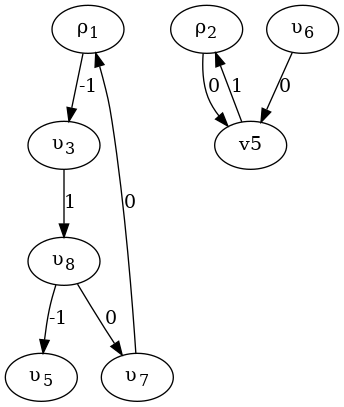
\includegraphics[width=0.3\linewidth]{figures/digraph.png}
% Generating the graph requires \usepackage{dot2texi} or \usepackage[pdf]{graphviz}
%\begin{dot2tex}[file=cstrnts,scale=0.6]
%digraph D {
%    p1 [label=<&rho;<SUB>1</SUB>>];
%    p2 [label=<&rho;<SUB>2</SUB>>];
%    v3 [label=<&upsilon;<SUB>3</SUB>>];
%    v4 [label=<&upsilon;<SUB>5</SUB>>];
%    v6 [label=<&upsilon;<SUB>6</SUB>>];
%    v7 [label=<&upsilon;<SUB>7</SUB>>];
%    v8 [label=<&upsilon;<SUB>8</SUB>>];
%    v7 -> p1 [label="0"];
%    v8 -> v7 [label="0"];
%    p2 -> v5 [label="0"];
%    v6 -> v5 [label="0"];
%    v8 -> v4 [label="-1"];
%    v3 -> v8 [label="1"];
%    p1 -> v3 [label="-1"];
%    v5 -> p2 [label="1"];
%}
%\end{dot2tex}
\caption{Example stage variable constraints as a weighted directed graph}
\label{fig:digraph}
\end{figure}

\textsc{RecCheckLoop} then calls $\textsc{RecCheck}(C, \rho_1, \set{\rho_1, \rho_2}, \upsilon_5)$. Following its steps, we have:
\begin{enumerate}
    \item $V^\iota = \set{\upsilon_7, \upsilon_8, \upsilon_3}$, and we add the constraints $C' = \rho_1 \sqsubseteq V^\iota$ (substaging each variable in $V^\iota$).
    \item It is evident that there are no negative-weight cycles in the constraint graph, so $V^- = \emptyset$.
    \item Nothing to be done.
    \item We have $\bigsqcup V^\neq = \set{\upsilon_5, \rho_2}$ and $\bigsqcup V^\iota = \set{\rho_1, \upsilon_3, \upsilon_8, \upsilon_7, \upsilon_4}$. Their intersection is empty, so we add no new constraints.
    \item There is no $\infty$ present, so $V^\bot = \emptyset$ and we return the constraints $C \cup C'$.
\end{enumerate}

\textsc{RecCheckLoop} executes without failure, so \texttt{defBody} indeed has type $\text{Nat}^{\rho_1} \to \text{Nat}^{\rho_2}$. Erasing this type to a global type for the global definition's type and to a position type for the fixpoint's type, the fully annotated program is then:

\begin{minted}[escapeinside=<>,mathescape=true]{coq}
Def example: Nat<$^\iota$> <$\to$> Nat<$^\iota$> <$\coloneqq$>
  fix<$_{\langle 1 \rangle, 1}$> <$\langle$>f: Nat<$^*$> <$\to$> Nat<$^*$> <$\coloneqq$>
    <$\lambda$>n: Nat. case<$_{\lambda x: \texttt{Nat}. \texttt{Nat}^\infty}$> n of
      <$\langle$>O <$\Rightarrow$> O,
       S <$\Rightarrow$> <$\lambda$>n': Nat. f n'<$\rangle \rangle$>.
\end{minted}

\section{Related Work}\label{sec:related}

This work is based on \CIChat \cite{cic-hat}, which describes CIC with sized types and a size inference algorithm. It assumes that position annotations are given by the user, requires each parameter of \coinductive types to be assigned polarities, and deals only with terms. We have added on top of it global declarations, constants and variables annotated by a vector of stage annotations, their $\delta$\-//$\Delta$\-/reductions, a let-in construction, an explicit treatment of mutually-defined \coinductive types and \cofixpoints, and an intermediate procedure \textsc{RecCheckLoop} to handle missing position annotations, while removing parameter polarities and subtyping rules based on these polarities.

The language \CIChatbar \cite{cic-hat-bar} is similar to \CIChat, described in greater detail, but with one major difference: \CIChatbar disallows stage variables in the bodies of abstractions, in the arguments of applications, and in case analysis branches, making \CIChatbar a strict subset of \CIChat. Any stage annotations found in these locations must be set to $\infty$. This solves the problem of knowing which stage annotations to use when using a variable defined as, for instance, an inductive type, simply by disallowing stage annotations in these definitions. However, this prevents us from using a variable as the \corecursive type of a \cofixpoint, and forces these types to be literal \coinductive types. In practice, such as in Coq's default theorems and libraries, aliases are often defined for \coinductive types, so we have worked around it with annotated variables and constants.

The implementation of \textsc{RecCheck} comes from \Fhat \cite{f-hat}, which is an extension of System F with type-based termination using sized types. Rules relating to coinductive constructions and cofixpoints come from the natural extension of \CChatomega \cite{cc-hat-omega}, which describes only infinite streams. Additionally, the judgement syntax for describing the size inference algorithm comes from \CChatomega and \CIChatl \cite{cic-hat-l}.

Whereas our successor sized types uses a size algebra that only has a successor operation, \textit{linear} sized types in \CIChatl extends the algebra by including stage annotations of the form $n \cdot S$, so that all annotations are of the form $n \cdot \upsilon + m$, where $m$ is the number of "hats". Unfortunately, this causes the time complexity of their \textsc{RecCheck} procedure to be worst-case doubly exponential in the number of stage variables. However, the set of typeable (and therefore terminating or productive) functions would be expanded even further; functions such as list-doubling could be typed as size-preserving in addition to being terminating. If successor sized types prove to be practically useable in Coq, augmenting the type system to linear sized types would be a viable consideration, depending on whether common programs in practice would cause worst-case behaviour. The most significant change required would be in \textsc{RecCheck}, which must then solve a set of constraints in Presburger arithmetic.

Well-founded sized types in \CIChatsub \cite{wellfounded} are yet another extension of successor sized types. The unpublished manuscript contains a type system, some metatheoretical results, and a size inference algorithm. In essence, it preserves subject reduction for coinductive constructions, and also expands the set of typeable functions.

\begin{figure}
    \centering
    
    \begin{mathpar}
    \infer[\defrule{size-var}]{
        \upsilon: \Size
    }{}
    
    \infer[\defrule{size-infty}]{
        \infty: \Size
    }{}
    
    \infer[\defrule{size-succ}]{
        \uparrow s: \Size
    }{
        s: \Size
    }
    
    \infer[\defrule{size-max}]{
        r \sqcup^s s : \Size
    }{
        r: \Size \\
        s: \Size
    }
    
    \infer[\defrule{size-lt}]{
        r: \Size
    }{
        r: \SizeLt s
    }
    
    \infer[\defrule{sizeuniv-size}]{
        \Size: \SizeUniv
    }{}
    
    \infer[\defrule{sizeuniv-size-lt}]{
        \SizeLt s: \SizeUniv
    }{
        s: \Size
    }
    \end{mathpar}
    
    \caption{Typing rules for sizes in Agda}
    \label{fig:agda-size}
\end{figure}

The proof assistant Agda implements sized types as user-provided size parameters, similar to type parameters. Correspondingly, sizes have the type \texttt{Size}, while \texttt{Size} itself has the type \texttt{SizeUniv}, which is its own type. \autoref{fig:agda-size} presents the typing rules for \texttt{Size}; the operator $\uparrow \cdot$ corresponds to our $\hat{\cdot}$, while $\cdot \sqcup^s \cdot$ takes the maximum of two sizes. Additionally, Agda defines the size constructor \texttt{Size<}, which allows the user to specify a size constraint $r \sqsubseteq s$ with the annotation $r: \text{Size<} s$. Whereas CIC$\widehat{~}\,$'s philosophy is to hide all size annotations from the user with a focus on size inference, Agda opts for allowing users to explicitly write size annotations and treat them almost like terms, yielding greater flexibility in deciding how things should be typed.

\section{Conclusion}
\label{sec:conclusion}
We have presented a design and implementation of sizes types for Coq.
Our work extends the core language and type checking algorithm of prior theoretical work on sized types for CIC with pragmatic features found in Gallina, such as global definitions, and extends the inference algorithm to infer sizes over completely unannotated Gallina terms to enable backward compatibility. We implement the design presented in this paper as an extension to Coq's kernel\cite{impl}. The design and implementation can be used alone or in conjunction with syntactic guard checking to maximize typeability and compatibility.

\clearpage

\bibliographystyle{ACM-Reference-Format}
\bibliography{main}

\clearpage

\appendix

\section{Supplementary Figures}\label{sec:figures}

\begin{figure*}
\centering

\begin{tabular}{l p{0.5\linewidth}}
    $\textsc{axiom} : U \to U$ & Produces type of universe\\
    $\textsc{rule} : U \times U \to U$ & Produces universe of product type given universe of argument and return types \\
    $\textsc{elim} : U \times U \times \mathcal{I} \to ()$ & Checks that given universe $\omega_k$ of \coinductive type $I_k$ of case analysis target can be eliminated to a type with given universe $\omega$; can fail \\
    $\cdot \preceq \cdot : T \times T \to \mathbb{P}(S \times S)$ & Checks subtypeability and produces a stage constraint set; can fail \\
    $\textsc{fresh} : \mathbb{N}^+ \to \vec{V}$ & Produces given number of fresh stage variables, putting them into $\mathcal{V}$ \\
    $\textsc{fresh*} : \mathbb{N}^+ \to \vec{P}$ & Produces given number of fresh position stage variables, putting them into both $\mathcal{V}$ and $\mathcal{P}$ \\
    $\textsc{inds} : \mathcal{I} \cup \mathcal{C} \to \mathbb{N}^+$ & Produces number of mutually-defined \coinductive types in definition to which given type or constructor belongs \\
    $\textsc{decompose} : T \times \mathbb{N}^0 \to \Delta \times T$ & Splits function type into given number of arguments and return type; can fail \\
    $\textsc{caseStage} : \mathcal{I} \times S \times \mathcal{V} \to \mathbb{P}(S \times S)$ & Given \coinductive type $I_k$, stage annotation $s$, and stage variable $\upsilon_k$, returns $\set{s \sqsubseteq \hat{\upsilon}_k}$ if $I_k$ is inductive and $\set{\hat{\upsilon}_k \sqsubseteq s}$ if $I_k$ is coinductive \\
    $\textsc{shift} : T \to T$ & Replaces each position stage annotation by successor \\
    $\textsc{setRecStars} : T^\circ \times \mathbb{N}^+ \to T^*$ & Given index $n$, annotates $n$th argument type $I$ and all other argument and return types with same type $I$ with position annotations; can fail \\
    $\textsc{setCorecStars} : T^\circ \to T^*$ & Annotates return argument type $I$ and all other argument types with same type $I$ with position annotations; can fail \\
    $\textsc{getRecVar} : T \times \mathbb{N}^+ \to \mathcal{P}$ & Given index $n$, retrieves position stage variable of $n$th argument type; can fail \\
    $\textsc{getCorecVar} : T \to \mathcal{P}$ & Retrieve position stage variable of return type; can fail \\
    $\textsc{getPosVars} : T \times T \to \mathcal{P}$ & Given function types $t, u$, returns stage variables from $t$ in same location as position stage variables in $u$; can fail \\
    $\textsc{RecCheckLoop} : C \times \mathbb{P}(\mathcal{V}) \times \vec{\mathcal{P}} \times \vec{T} \times \vec{T} \to C$ & Calls \textsc{RecCheck} recursively, shrinking $\mathcal{P}$ each time; can fail via \textsc{RecCheck} \\
    $\textsc{RecCheck} : C \times \mathcal{P} \times \mathbb{P}(\mathcal{P}) \times \mathbb{P}(\mathcal{V}) \to C$ & Checks termination and productivity using stage constraints, returning a new set of constraints; can fail
\end{tabular}

\caption{Summary of metafunctions used in the size inference algorithm}
\label{fig:inference-metafunctions}
\end{figure*}

\autoref{fig:inference-metafunctions} lists the various metafunctions introduced in \autoref{sec:algorithm} with their signatures and a short description.

\begin{comment}
\section{Simplified \titlelang}
We present a simplified variant of \lang without mutually-defined \coinductive types and mutual \cofixpoints. While adhering less to Gallina, this is closer to \CIChatbar and \CIChat, and is easier to reason about. Going from the proper \lang to the simplified \lang is simple, and we provide the simplified variant explicitly for convenience. The modified portions of the syntax of terms and \coinductive definitions for simplified \lang are given in \autoref{fig:simpl-terms} and \autoref{fig:simpl-inductives}.

\begin{figure}
\centering
\begin{align*}
T[\alpha] &\Coloneqq \dots \\
    &\mid \fix*{n}{\mathcal{X}}{T^*}{T[\alpha]} \\
    &\mid \cofix*{}{\mathcal{X}}{T^*}{T[\alpha]}
\end{align*}
\caption{Syntax of \lang terms with no mutual \cofixpoints (excerpt)}
\label{fig:simpl-terms}
\end{figure}

\begin{figure}
\centering
\begin{align*}
\textit{Ind} &\Coloneqq \mathcal{I}: \Pi\Delta . \Pi\Delta^\infty . U \coloneqq \langle \mathcal{C}: \Pi\Delta^\infty . \mathcal{I}\ \overline{\mathcal{X}}\ \overline{T^\infty} \rangle
\end{align*}
\begin{equation*}
I: \Pi\Delta_p. \Pi\Delta_i . \varw_I \coloneqq \langle c_j: \Pi\Delta_j . I\ \dom{\Delta_p}\ \overline{t}_j \rangle
\end{equation*}
\caption{(Co)inductive definitions with no mutually-defined inductive types}
\label{fig:simpl-inductives}
\end{figure}

We give the corresponding typing rules for case expressions and \cofixpoints in \autoref{fig:simpl-typing}, as well as the required metafunctions in \autoref{fig:simpl-metafunctions}. The main differences to note are that only a single stage annotation is passed to the metafunctions, and we no longer need indices to differentiate between different mutually-defined \coinductive types in the case rule or to differentiate between different mutual \cofixpoint definitions in the (co)fix rules.

\begin{figure}
\centering
\begin{align*}
    \indtype{\Sigma}{I} &=
        \Pi \Delta_p . \Pi \Delta_i . \varw_I \\
    \constrtype{\Sigma}{c_\ell}{s} &=
        \Pi \Delta_p . \Pi \Delta_\ell [I^\infty \coloneqq I^s] . I^{\hat{s}}\ \dom{\Delta_p}\ \overline{t}_\ell \\
    \motivetype{\Sigma}{\overline{p}}{\varw}{I^s} &=
        \Pi \Delta_i[\dom{\Delta_p} \coloneqq \overline{p}] . \Pi \_ : I^s\ \overline{p}\ \dom{\Delta_i} . \varw \\
    \branchtype{\Sigma}{\overline{p}}{c_\ell}{s}{\wp} &=
        \Pi \Delta_\ell [I^\infty \coloneqq I^s][\dom{\Delta_p} \coloneqq \overline{p}] . \wp\ \overline{t}_\ell\ (c_\ell\ \overline{p}\ \dom{\Delta_\ell})
\end{align*}
\begin{displaymath}
    \textit{where}\;\:
    \ell \in \overline{\jmath},
    \big(I: \Pi\Delta_p . \Pi\Delta_i . \varw_I \coloneqq \langle c_j : \Pi \Delta_j . I_j\ \_\ \overline{t}_j \rangle \big) \in \Sigma
\end{displaymath}
\caption{Metafunctions for typing rules}
\label{fig:simpl-metafunctions}
\end{figure}

\begin{figure}
\centering
\begin{mathpar}
    \inferrule*[right=(case)]{
        \sgg \vdash e : I^{\hat{s}}\ \overline{p}\ \overline{a} \\
        \indtype{\Sigma}{I} = \Pi \_ . \Pi \_ . \varw_I \qquad (\varw_I, \varw, I) \in \text{Elims} \\\\
        \sgg \vdash \wp : \motivetype{\Sigma}{\overline{p}}{\varw}{I^{\hat{s}}} \\
        \sgg \vdash e_j : \branchtype{\Sigma}{\overline{p}}{c_j}{s}{\wp}
    }{
        \sgg \vdash \caseof{|\wp|}{e}{c_j}{e_j} : \wp\overline{a}e
    }
    \hva \and
    \inferrule*[right=(fix)]{
        t \approx \Pi \Delta_1 . \Pi x : I^\upsilon\ \overline{a}. \Pi \Delta_2 . u \\
        \|\Delta_1\| = n - 1 \\
        \upsilon \pos \Delta_1, \Delta_2, u \\
        \upsilon \notin \SV{\Gamma, \overline{a}, e} \\
        \upsilon, \lfloor s \rfloor \in \mathcal{P} \\
        \sgg \vdash t : \varw \\
        \sgg (f : t) \vdash e : t[\upsilon \coloneqq \hat{\upsilon}]
    }{
        \sgg \vdash \fix*{n}{f}{|t|^*}{e} : t[\upsilon \coloneqq s]
    }
    \hva \and
    \inferrule*[right=(cofix)]{
        t \approx \Pi \Delta . I^\upsilon\ \overline{a} \\
        \upsilon \neg \Delta \\
        \upsilon \notin \SV{\Gamma, \overline{a}, e} \\
        \upsilon, \lfloor s \rfloor \in \mathcal{P} \\
        \sgg \vdash t : \varw \\
        \sgg (f : t) \vdash e : t[\upsilon \coloneqq \hat{\upsilon}]
    }{
        \sgg \vdash \cofix*{}{f}{|t|^*}{e_k} : t[\upsilon \coloneqq s]
    }
\end{mathpar}
\caption{Typing rules (excerpt)}
\label{fig:simpl-typing}
\end{figure}

Finally, we give the corresponding size inference algorithm for these terms in \autoref{fig:simpl-algorithm}. Again, we do away with some of the indices, and \textsc{RecCheckLoop} now takes a single stage annotation, a single term, and a single type. The modified version of \textsc{RecCheckLoop} is provided in \autoref{fig:simpl-helpers}

\begin{figure}
\centering
\begin{mathpar}
\inferrule*[right=(a-case)]{
    \cgg \vdash e^\circ \rightsquigarrow C_1, e \Rightarrow^* I^s\ \overline{p}\ \overline{a} \\
    C_1, \Gamma_G, \Gamma \vdash \wp^\circ \rightsquigarrow C_2, \wp \Rightarrow t_p \\
    \Pi \_ . \Pi \Delta_i . \varw_I = \indtype{\Sigma}{I} \\
    (\_, \varw) = \decompose{t_p}{\|\Delta_i\| + 1} \\
    \elim{\varw_I}{\varw}{I} \\
    \upsilon = \fresh{1} \\
    C_3 = \caseStage{I^s}{\hat{\upsilon}} \\
    C_4 = t_p \preceq \motivetype{\Sigma}{\overline{p}}{\varw}{I^{\hat{\upsilon}}} \\
    C_5 = C_2 \cup C_3 \cup C_4 \\
    C_5, \Gamma_G, \Gamma \vdash e^\circ_j \Leftarrow \branchtype{\Sigma}{\overline{p}}{c_j}{\upsilon}{\wp} \rightsquigarrow C_{6j}, e_j \\
    C_6 = \textstyle\bigcup_j C_{6j}
}{
    \cgg \vdash \caseof{\wp^\circ}{e^\circ}{c_j}{e_j^\circ} \rightsquigarrow C_6, \caseof{|\wp|}{e}{c_j}{e_j} \Rightarrow \wp\overline{a}e
}
\hva \and
\inferrule*[right=(a-fix)]{
    \cgg \vdash t^\circ \rightsquigarrow \_, \_ \Rightarrow \_ \\\\
    \cgg \vdash \setrecstars{t^\circ}{n} \rightsquigarrow C_1, t \Rightarrow^* \varw \\\\
    C_1, \Gamma_G, \Gamma(f : t) \vdash e^\circ \Leftarrow  \shift{t} \rightsquigarrow C_2, e \\
    C_3 = \RecCheckLoop{C_2}{\getrecvar{t}{n}}{t}{e}
}{
    \cgg \vdash \fix*{n}{f_k}{t^\circ}{e} \rightsquigarrow C_3, \fix*{n}{f}{|t|^*}{e} \Rightarrow t
}
\hva \and
\inferrule*[right=(a-fix)]{
    \cgg \vdash t^\circ \rightsquigarrow \_, \_ \Rightarrow \_ \\\\
    \cgg \vdash \setcorecstars{t^\circ} \rightsquigarrow C_1, t \Rightarrow^* \varw \\\\
    C_1, \Gamma_G, \Gamma(f : t) \vdash e^\circ \Leftarrow  \shift{t} \rightsquigarrow C_2, e \\
    C_3 = \RecCheckLoop{C_2}{\getcorecvar{t}}{t}{e}
}{
    \cgg \vdash \cofix*{}{f_k}{t^\circ}{e} \rightsquigarrow C_3, \cofix*{}{f}{|t|^*}{e} \Rightarrow t
}
\end{mathpar}
\caption{Size inference algorithm (excerpt)}
\label{fig:simpl-algorithm}
\end{figure}
\begin{figure}
\centering

\begin{minted}[escapeinside=<>,mathescape=true]{ocaml}
                let rec RecCheckLoop <$C_2$> <$\rho$> <$t$> <$e$> =
                  try let pv = <$\texttt{PV}$> <$t$> in
                      let sv = (<$\texttt{SV}$> <$t$> <$\cup$> <$\texttt{SV}$> <$e$>) <$\setminus$> pv in
                      RecCheck <$C_2$> <$\rho$> pv sv
                  with RecCheckFail <$V$> ->
                      <$\mathcal{P}$> := <$\mathcal{P} \setminus V$>;
                      RecCheckLoop <$C_2$> <$\rho$> <$t$> <$e$>
\end{minted}

\caption{Modified pseudocode implementation of \textsc{RecCheckLoop}}
\label{fig:simpl-helpers}
\end{figure}
\end{comment}
\end{document}
